%%
% A header that lets you compile a chapter by itself, or inside a larger document.
% Adapted from http://stackoverflow.com/questions/3655454/conditional-import-in-latex
%
%
%Use \inbpdocument and \outbpdocument in your individual files, in place of \begin{document} and \end{document}. In your main file, put in a \def \ismaindoc {} before including or importing anything.
%
% David Duvenaud
% June 2011
% 
% ======================================
%
%


\ifx\ismaindoc\undefined
	\newcommand{\inbpdocument}{
		\def \ismaindoc {}
		% Use this header if we are compiling by ourselves.
		\documentclass[a4paper,11pt]{common/PhDThesisPSnPDF}
		\usepackage[round]{natbib} 
\usepackage{hyperref} 
\usepackage{url} %tablerules
\usepackage{cleveref}
\usepackage{soul}


%\usepackage{draftwatermark}
%\SetWatermarkLightness{0.95}

% ******************************************************************************
% ****************************** Custom Margin *********************************

% Add `custommargin' in the document class options to use this section
% Set {innerside margin / outerside margin / topmargin / bottom margin}  and
% other page dimensions

\ifsetMargin
\else
    \RequirePackage[left=37mm,right=30mm,top=35mm,bottom=30mm]{geometry}
    \setFancyHdr % To apply fancy header after geometry package is loaded
\fi


%\chead{Unfinished draft}
\cfoot{\texttt{Unfinished draft - compiled on \today{} at \currenttime}}

% *****************************************************************************
% ******************* Fonts (like different typewriter fonts etc.)*************

% Add `customfont' in the document class option to use this section

\ifsetFont
\else
    % Set your custom font here and use `customfont' in options. Leave empty to
    % load computer modern font (default LaTeX font).  

    \RequirePackage{libertine} 
\fi



% Add appendices
\RequirePackage[title,titletoc]{appendix}

% changes the default name `Bibliography` -> `References'
%\renewcommand{\bibname}{References}


% *****************************************************************************
% *************** Changing the Visual Style of Chapter Headings ***************
% Uncomment the section below. Requires titlesec package.

%\RequirePackage{titlesec}
%\newcommand{\PreContentTitleFormat}{\titleformat{\chapter}[display]{\scshape\Large}
%{\Large\filleft{\chaptertitlename} \Huge\thechapter}
%{1ex}{}
%[\vspace{1ex}\titlerule]}
%\newcommand{\ContentTitleFormat}{\titleformat{\chapter}[display]{\scshape\huge}
%{\Large\filleft{\chaptertitlename} \Huge\thechapter}{1ex}
%{\titlerule\vspace{1ex}\filright}
%[\vspace{1ex}\titlerule]}
%\newcommand{\PostContentTitleFormat}{\PreContentTitleFormat}
%\PreContentTitleFormat


% *****************************************************************************
% **************************** Custom Packages ********************************
% *****************************************************************************


% ************************* Algorithms and Pseudocode **************************

%\usepackage{algpseudocode} 


% ********************Captions and Hyperreferencing / URL **********************

% Captions: This makes captions of figures use a boldfaced small font. 
%\RequirePackage[small,bf]{caption}

\RequirePackage[labelsep=space,tableposition=top]{caption} 
\renewcommand{\figurename}{Fig.} %to support older versions of captions.sty
\captionsetup{belowskip=12pt,aboveskip=4pt}

% ************************ Formatting / Footnote *******************************

%\usepackage[perpage]{footmisc} %Range of footnote options 


% ****************************** Line Numbers **********************************

%\RequirePackage{lineno}
%\linenumbers

% ************************** Graphics and figures *****************************

\usepackage{rotating}
\usepackage{lscape} 
%\usepackage{wrapfig}
%\usepackage{float}
%subfigures deprecated
%\usepackage{subfigure}
%use subcaption instead
\usepackage[labelfont=bf,labelsep=period,justification=raggedright]{caption}
\usepackage{subcaption}
%\usepackage{subfig} %note: subfig must be included after the `caption` package. 


% ********************************* Table **************************************

%for table cell with diagonal division
%\usepackage{multicol}
\usepackage{multirow}
\usepackage{tabularx}
\usepackage{slashbox}
\usepackage{longtable} 
\usepackage{booktabs}
\usepackage{tabu}
\usepackage{xcolor,colortbl}



% ***************************** Math and SI Units ******************************

\usepackage{amsthm}
\usepackage{amsfonts}
\usepackage{amsmath}
\usepackage{amssymb}
\usepackage{textcomp}
% degree celsius
%\usepackage{gensymb}
%percentages, microliters, nanograms etc
\usepackage{siunitx}
\DeclareSIUnit[number-unit-product={}]\unit{U}


% ******************************************************************************
% ************************* User Defined Commands ******************************
% ******************************************************************************

% *********** To change the name of Table of Contents / LOF and LOT ************

%\renewcommand{\contentsname}{My Table of Contents}
%\renewcommand{\listfigurename}{My List of Figures}
%\renewcommand{\listtablename}{My List of Tables}


% ********************** TOC depth and numbering depth *************************

%\setcounter{secnumdepth}{2}
%\setcounter{tocdepth}{2}

% ******************************* Nomenclature *********************************

% To change the name of the Nomenclature section, uncomment the following line

%\renewcommand{\nomname}{Symbols}


% ********************************* Appendix ***********************************

% The default value of both \appendixtocname and \appendixpagename is `Appendices'. These names can all be changed via: 

%\renewcommand{\appendixtocname}{List of appendices}
%\renewcommand{\appendixname}{Appndx}


%%% Packages
% Use Charter font.
%\usepackage{charter}
% for line spacing
\usepackage{setspace}
\usepackage{xspace}
% Use PDF output.
%\usepackage[pdftex]{color,graphicx}
% The output should be wide.
%\usepackage{a4wide}
%\usepackage[a4paper]{geometry}
%\usepackage[text={7.5in,9in},centering]{geometry}
%\usepackage[cm]{fullpage}
%for definition list
\usepackage{enumitem}
%puts silly zeroes in section names
%\usepackage{fancyhdr}
%for code snippets
%\usepackage{float}
%\floatstyle{ruled}
%\newfloat{program}{thp}{lop}
%\floatname{program}{Code snippet} 
\usepackage{tikz}
\usetikzlibrary{shapes,arrows,calc,through,backgrounds,decorations.pathmorphing,shadows} 
%\usepackage[active,tightpage]{preview} 
\usepackage[french, greek, english]{babel}
%input encoding
%\usepackage[iso-8859-7]{inputenc}
%\usepackage[latin1]{inputenc}
%output encoding
\usepackage[T1]{fontenc}
\selectlanguage{english} 
% Pour la dedicace
\usepackage{frcursive} 
%side caption: SCfigure
%\usepackage{sidecap}
%\usepackage[table]{xcolor}
%\usepackage[graphics,tightpage,active]{preview}
%\PreviewEnvironment{tikzpicture}
%\PreviewEnvironment{equation}
%\PreviewEnvironment{equation*}
%\newlength{\imagewidth}
%\newlength{\imagescale}
%\pagestyle{empty}
%\thispagestyle{empty}
%\usepackage{standalone} 
\usepackage[section,subsection,subsubsection]{extraplaceins} 
\usepackage{authblk} 
\usepackage{graphicx} 
%unicode support
\usepackage[utf8]{inputenc} 
%multiple indices
\usepackage{multind}
%glossary
\usepackage[acronym]{glossaries}

\usepackage{datetime}
\renewcommand{\tabularxcolumn}[1]{>{\arraybackslash}m{#1}}
\usepackage{relsize}
\usepackage{nicefrac}
\usepackage{nth}
\usepackage{array}




		% All my custom preamble stuff.  Shouldn't overlap with anything in official-preamble


% Paths to figure and table directories.
\newcommand{\symmetryfigsdir}{figures/symmetries}
\newcommand{\topologyfiguresdir}{figures/topology}
\newcommand{\infinitefiguresdir}{figures/infinite}
\newcommand{\grammarfiguresdir}{figures/grammar}
\newcommand{\introfigsdir}{figures/intro}
\newcommand{\gplvmfiguresdir}{figures/gplvm}
\newcommand{\warpedfiguresdir}{figures/warped-mixtures}
\newcommand{\deeplimitsfiguresdir}{figures/deep-limits}
\newcommand{\quadraturefigsdir}{figures/quadrature}
\newcommand{\additivefigsdir}{figures/additive}
\newcommand{\decompfigsdir}{figures/decomp}
\newcommand{\examplefigsdir}{figures/worked-example}


\usepackage{bm}  % for warped mixtures - is this necessary?
\usepackage{booktabs}
\usepackage{tabularx}
\usepackage{multirow}
\usepackage{datetime}
\renewcommand{\tabularxcolumn}[1]{>{\arraybackslash}m{#1}}
\usepackage{relsize}
\usepackage{graphicx}
\usepackage{amsmath,amssymb,textcomp}
\usepackage{nicefrac}
\usepackage{amsthm}
\usepackage{tikz}
\usetikzlibrary{arrows}
\usetikzlibrary{calc}
\usepackage{nth}
\usepackage{rotating}
\usepackage{array}
\usepackage[hyperpageref]{backref}


\def\foo{\hspace{\fill}\mbox{}\linebreak[0]\hspace*{\fill}}
\renewcommand*{\backref}[1]{}
\renewcommand*{\backrefalt}[4]{%
\ifcase #1 %
%
\or
\foo(page #2)%
\else
\foo(pages #2)%
\fi
}

\usepackage{cleveref}
\crefname{equation}{equation}{equations}


%% For submission, make all render blank.
%%%%%%%%%%%%%%%%%%%%%%%%%%%%%%%%%%%%%%%%%%%%%%%%%%%%%%%%%%
%%%% EDITING HELPER FUNCTIONS  %%%%%%%%%%%%%%%%%%%%%%%%%%%
%%%%%%%%%%%%%%%%%%%%%%%%%%%%%%%%%%%%%%%%%%%%%%%%%%%%%%%%%%

%% NA: needs attention (rough writing whose correctness needs to be verified)
%% TBD: instructions for how to fix a gap ("Describe the propagation by ...")
%% PROBLEM: bug or missing crucial bit 

%% use \fXXX versions of these macros to put additional explanation into a footnote.  
%% The idea is that we don't want to interrupt the flow of the paper or make it 
%% impossible to read because there are a bunch of comments.

%% NA's (and TBDs, those less crucially) should be written so 
%% that they flow with the text.

\definecolor{WowColor}{rgb}{.75,0,.75}
\definecolor{SubtleColor}{rgb}{0,0,.50}

% inline
\newcommand{\NA}[1]{\textcolor{SubtleColor}{ {\tiny \bf ($\star$)} #1}}
\newcommand{\LATER}[1]{\textcolor{SubtleColor}{ {\tiny \bf ($\dagger$)} #1}}
\newcommand{\TBD}[1]{\textcolor{SubtleColor}{ {\tiny \bf (!)} #1}}
\newcommand{\PROBLEM}[1]{\textcolor{WowColor}{ {\bf (!!)} {\bf #1}}}

% as margin notes

\newcounter{margincounter}
\newcommand{\displaycounter}{{\arabic{margincounter}}}
\newcommand{\incdisplaycounter}{{\stepcounter{margincounter}\arabic{margincounter}}}

\newcommand{\fTBD}[1]{\textcolor{SubtleColor}{$\,^{(\incdisplaycounter)}$}\marginpar{\tiny\textcolor{SubtleColor}{ {\tiny $(\displaycounter)$} #1}}}

\newcommand{\fPROBLEM}[1]{\textcolor{WowColor}{$\,^{((\incdisplaycounter))}$}\marginpar{\tiny\textcolor{WowColor}{ {\bf $\mathbf{((\displaycounter))}$} {\bf #1}}}}

\newcommand{\fLATER}[1]{\textcolor{SubtleColor}{$\,^{(\incdisplaycounter\dagger)}$}\marginpar{\tiny\textcolor{SubtleColor}{ {\tiny $(\displaycounter\dagger)$} #1}}}

%\renewcommand{\LATER}[1]{}
%\renewcommand{\fLATER}[1]{}
%\renewcommand{\TBD}[1]{}
%\renewcommand{\fTBD}[1]{}
%\renewcommand{\PROBLEM}[1]{}
%\renewcommand{\fPROBLEM}[1]{}
%\renewcommand{\NA}[1]{}


% HUMBLE WORDS: shown slightly smaller when in normal text
% Thanks to Christian Steinruecken!

% HUMBLE WORDS: shown slightly smaller when in normal text
%
\makeatletter%
%\def\@humbleformat#1{{\fontsize{}{1em}\selectfont #1}}
%\def\@humbleformat#1{\textsmaller{#1}}%
\newlength{\nonHumbleHeight}
\def\@humbleformat#1{{\settoheight{\nonHumbleHeight}{#1}\resizebox{!}{0.94\nonHumbleHeight}{#1}}}%
\def\@idxhumbleformat#1{{\relscale{0.95}{#1}}}%
%\def\@humbleformat#1{{#1}}%
\def\declareHumble#1#2{%
  \expandafter\def\csname #1\endcsname{\@humbleformat{#2}}%
  \expandafter\def\csname s#1\endcsname{{#2}}%
  \expandafter\def\csname idx#1\endcsname{{\@idxhumbleformat{#2}}}%
}%
\def\humble#1{\@humbleformat{#1}}%
\def\idxhumble#1{\@idxhumbleformat{#1}}%
\makeatother%

% Convenient indexing for humble abbreviations
\def\humbleindex#1#2{\index{#1@\idxhumble{#1}}}



% TODO: Clean up duplicates
\declareHumble{ANOVA}{ANOVA}
\declareHumble{ARD}{ARD}
\declareHumble{BIC}{BIC}
\declareHumble{BMC}{BMC}
\declareHumble{bq}{BQ}
\declareHumble{CRP}{CRP}
\declareHumble{dirpro}{DP}
\declareHumble{HDMR}{HDMR}
\declareHumble{GAM}{GAM}
\declareHumble{GEM}{GEM}
\declareHumble{GMM}{GMM}
\declareHumble{gplvm}{GP-LVM}
\declareHumble{gpml}{GPML}
\declareHumble{GPML}{GPML}
\declareHumble{gprn}{GPRN}
\declareHumble{gpt}{GP}
\declareHumble{gp}{GP}
\declareHumble{HKL}{HKL}
\declareHumble{HMC}{HMC}
\declareHumble{ibp}{IBP}
\declareHumble{iGMM}{iGMM}
\declareHumble{iwmm}{iWMM}
\declareHumble{kCP}{CP}
\declareHumble{kCW}{CW}
\declareHumble{kC}{C}
\declareHumble{KDE}{KDE}
\declareHumble{kLin}{Lin}
\declareHumble{KPCA}{KPCA}
\declareHumble{kPer}{Per}
\declareHumble{kRQ}{RQ}
\declareHumble{kSE}{SE}
\declareHumble{kWN}{WN}
\declareHumble{Lin}{Lin}
\declareHumble{LBFGS}{L-BFGS}
\declareHumble{mcmc}{MCMC}
\declareHumble{MKL}{MKL}
\declareHumble{MLP}{MLP}
\declareHumble{MSE}{MSE}
\declareHumble{Per}{Per}
\declareHumble{RMSE}{RMSE}
\declareHumble{RQ}{RQ}
\declareHumble{SBQ}{SBQ}
\declareHumble{seard}{SE-ARD}
\declareHumble{sefull}{SE-\textnormal{full}}
\declareHumble{SEGP}{SE-GP}
\declareHumble{SE}{SE}
\declareHumble{SNR}{SNR}
\declareHumble{SSANOVA}{SS-ANOVA}
\declareHumble{SVM}{SVM}

\newcommand{\kSig}{\boldsymbol\sigma}

\def\subexpr{{\cal S}}
\def\baseker{{\cal B}}
\def\numWinners{k}

\def\ie{i.e.\ }
\def\eg{e.g.\ }
\def\etc{etc.\ }
\let\oldemptyset\emptyset
\let\emptyset 0


% For tikz figures in deep limits
\newcommand{\numdims}[0]{3}
\newcommand{\numhidden}[0]{4}
\newcommand{\upnodedist}[0]{0.6cm}
\newcommand{\bardist}[0]{\hspace{-0.2cm}}

% Unify notation between neural-net land and GP-land.
\newcommand{\hphi}{h}
\newcommand{\hPhi}{\vh}
\newcommand{\walpha}{w}
\newcommand{\wboldalpha}{\bw}
\newcommand{\wcapalpha}{\vW}
\newcommand{\lengthscale}{w}

\newcommand{\layerindex}{\ell}



\newcommand{\gpdrawbox}[1]{
\setlength\fboxsep{0pt}
\hspace{-0.15in} 
\fbox{
\includegraphics[width=0.464\columnwidth]{\deeplimitsfiguresdir/deep_draws/deep_gp_sample_layer_#1}
}}



\newcommand{\procedurename}{ABCD}
\newcommand{\genText}[1]{{\sf #1}}



\newcommand{\asdf}{$^{\textnormal{th}}$}

\newcommand{\binarysum}{\sum_{\bf{x} \in \{0,1\}^D}}
\newcommand{\expect}{\mathbb{E}}
\newcommand{\expectargs}[2]{\mathbb{E}_{#1} \left[ {#2} \right]}
\newcommand{\var}{\mathbb{V}}
\newcommand{\varianceargs}[2]{\mathbb{V}_{#1} \left[ {#2} \right]}
\newcommand{\cov}{\operatorname{cov}}
\newcommand{\Cov}{\operatorname{Cov}}
\newcommand{\covargs}[2]{\cov \left[ {#1}, {#2} \right]}
\newcommand{\variance}{\mathbb{V}}
\newcommand{\vecop}[1]{\operatorname{vec} \left( {#1} \right)}

\newcommand{\covarianceargs}[2]{\Cov_{#1} \left[ {#2} \right]}
\newcommand{\colvec}[2]{\left[ \begin{array}{c} {#1} \\ {#2} \end{array} \right]}
\newcommand{\tbtmat}[4]{\left[ \begin{array}{cc} {#1} & {#2} \\ {#3} & {#4} \end{array} \right]}

%\newcommand{\covskinny}[2]{\var\!\left(#1\middle\vert#2\right)} 

\newcommand{\acro}[1]{{\humble{#1}}}
%\newcommand{\vect}[1]{\boldsymbol{#1}}
\newcommand{\vect}[1]{{\bf{#1}}}
\newcommand{\mat}[1]{\mathbf{#1}}
\newcommand{\pderiv}[2]{\frac{\partial #1}{\partial #2}}
\newcommand{\npderiv}[2]{\nicefrac{\partial #1}{\partial #2}}

\newcommand{\pha}{^{\phantom{:}}}

\newcommand{\argmin}{\operatornamewithlimits{argmin}}
\newcommand{\argmax}{\operatornamewithlimits{argmax}}

% The following designed for probabilities with long arguments

\newcommand{\Prob}[2]{P\!\left(\,#1\;\middle\vert\;#2\,\right)}
\newcommand{\ProbF}[3]{P\!\left(\,#1\!=\!#2\;\middle\vert\;#3\,\right)}
\newcommand{\p}[2]{p\!\left(#1\middle\vert#2\right)}
\newcommand{\po}[1]{p\!\left(#1\right)}
\newcommand{\pF}[3]{p\!\left(\,#1\!=\!#2\;\middle\vert\;#3\,\right)} 
\newcommand{\mean}[2]{{m}\!\left(#1\middle\vert#2\right)}



\newcommand{\valpha}{\boldsymbol{\alpha}}
\newcommand{\va}{\vect{a}}
\newcommand{\vA}{\vect{A}}
\newcommand{\vB}{\mat{B}}
\newcommand{\vb}{\vect{b}}
\newcommand{\vC}{\mat{C}}
\newcommand{\vc}{\vect{c}}
\newcommand{\vecf}{\boldsymbol{f}}
\newcommand{\vell}{\vect{\ell}}
\newcommand{\vepsilon}{\boldsymbol{\epsilon}}
\newcommand{\veps}{\boldsymbol{\epsilon}}
\newcommand{\ve}{\boldsymbol{\epsilon}}
\newcommand{\vf}{\vecf}
\newcommand{\vg}{\vect{g}}
\newcommand{\vh}{\vect{h}}
\newcommand{\vI}{\mat{I}}
\newcommand{\vK}{\mat{K}}
\newcommand{\vk}{\vect{k}}
\newcommand{\vL}{\mat{L}}
\newcommand{\vl}{\vect{l}}
\newcommand{\vmu}{\boldsymbol{\mu}}
\newcommand{\vone}{\vect{1}}
\newcommand{\vphi}{\boldsymbol{\phi}}
\newcommand{\vpi}{\boldsymbol{\pi}}
\newcommand{\vq}{\vect{q}}
\newcommand{\vR}{\mat{R}}
\newcommand{\vr}{\vect{r}}
\newcommand{\vsigma}{\boldsymbol{\sigma}}
\newcommand{\vSigma}{\mat{\Sigma}}
\newcommand{\vS}{\mat{S}}
\newcommand{\vs}{\vect{s}}
\newcommand{\vtheta}{\boldsymbol{\theta}}
\newcommand{\vu}{\vect{u}}
\newcommand{\vV}{\mat{V}}
\newcommand{\vW}{\mat{W}}
\newcommand{\vw}{\vect{w}}
\newcommand{\vX}{\mat{X}}
\newcommand{\vx}{\vect{x}}
\newcommand{\vY}{\mat{Y}}
\newcommand{\vy}{\vect{y}}
\newcommand{\vzero}{\vect{0}}
\newcommand{\vZ}{\mat{Z}}
\newcommand{\vz}{\vect{z}}


\newcommand{\netweights}{\alpha}
\newcommand{\vnetweights}{\valpha}

\newcommand{\He}{\mathcal{H}}
\newcommand{\normx}[2]{\left\|#1\right\|_{#2}}
\newcommand{\Hnorm}[1]{\normx{#1}{\He}}
\newcommand{\mmd}{{\rm MMD}}


\newcommand{\mf}{\bar{\vf}}

%\newcommand{\mf}{\mu} %{\bar{\ell}}
\newcommand{\lf}{f} % Likelihood function
\newcommand{\st}{_\star}

% from simpler log-bq writeup
\newcommand{\lftwo}{{\log \ell}}
\newcommand{\mftwo}{{\bar \ell}}
\newcommand{\loggp}{{\log\acro{GP}}}%| \bX, \vy )}}
\newcommand{\loggpdist}{{\acro{GP}(\lftwo)}}%| \vX, \vy )}}


\newcommand{\inv}{^{{\mathsmaller{-1}}}}
\newcommand{\tohalf}{^{{\mathsmaller{\nicefrac{1}{2}}}}}

\newcommand{\Normal}{\mathcal{N}}
\newcommand{\N}[3]{\mathcal{N}\!\left(#1 \middle| #2,#3\right)}
\newcommand{\Nt}[2]{\mathcal{N}\!\left(#1,#2\right)}
\newcommand{\NT}[2]{\mathcal{N}\!\left(#1,#2\right)}
\newcommand{\GPdist}[3]{\mathcal{GP}\!\left(#1 \, \middle| \, #2, #3 \right)}
\newcommand{\bN}[3]{\mathcal{N}\big(#1 \middle| #2,#3\big)}
\newcommand{\boldN}[3]{\text{\textbf{\mathcal{N}}}\big(#1;#2,#3\big)}
\newcommand{\ones}[1]{\mat{1}_{#1}}
\newcommand{\eye}[1]{\mat{E}_{#1}}
\newcommand{\tra}{^{\mathsf{T}}}
%\newcommand{\tra}{^{\top}}
%\mathsf{T}
\newcommand{\trace}{\operatorname{tr}}
\newcommand{\shift}{\operatorname{shift}}
\renewcommand{\mod}{\operatorname{mod}}
\newcommand{\deq}{:=}
\newcommand{\oneofk}{\operatorname{one-of-k}}
%\newcommand{\degree}{^\circ}

\newcommand{\GPt}[2]{\mathcal{GP}\!\left(#1,#2\right)}
%\newcommand{\GPt}[2]{\gp\!\left(#1,#2\right)}

\DeclareMathOperator{\tr}{tr}
\DeclareMathOperator{\chol}{chol}
\DeclareMathOperator{\diag}{diag}

\newenvironment{narrow}[2]{%
  \begin{list}{}{%
  \setlength{\topsep}{0pt}%
  \setlength{\leftmargin}{#1}%
  \setlength{\rightmargin}{#2}%
  \setlength{\listparindent}{\parindent}%
  \setlength{\itemindent}{\parindent}%
  \setlength{\parsep}{\parskip}}%
\item[]}{\end{list}}



\newcommand{\dist}{\ \sim\ }
\def\given{\,|\,}

% Table stuff
\newcolumntype{C}[1]{>{\centering\let\newline\\\arraybackslash\hspace{0pt}}m{#1}}
\newcolumntype{L}[1]{>{\raggedright\let\newline\\\arraybackslash\hspace{0pt}}m{#1}}
\newcolumntype{R}[1]{>{\raggedleft\let\newline\\\arraybackslash\hspace{0pt}}m{#1}}


\def\ie{i.e.\ }
\def\eg{e.g.\ }
\def\iid{i.i.d.\ }
%\def\simiid{\sim_{\mbox{\tiny iid}}}
\def\simiid{\overset{\mbox{\tiny iid}}{\sim}}
\def\simind{\overset{\mbox{\tiny \textnormal{ind}}}{\sim}}
\def\eqdist{\stackrel{\mbox{\tiny d}}{=}}
%\newcommand{\distas}[1]{\mathbin{\overset{#1}{\kern \z@ \sim}}}
%TODO: fix this - it worked outside the thesis!
\newcommand{\distas}[1]{\mathbin{\overset{#1}{\sim}}}

\def\Reals{\mathbb{R}}

\def\Uniform{\mbox{\rm Uniform}}
\def\Bernoulli{\mbox{\rm Bernoulli}}
\def\GP{\mathcal{GP}}
\def\GPLVM{\mathcal{GP-LVM}}




% Kernel stuff

\def\iva{\vect{\inputVar}}
\def\ivaone{\inputVar}
\def\inputVar{x}
\def\InputVar{X}
\def\InputSpace{\mathcal{X}}
\def\outputVar{y}
\def\OutputSpace{\mathcal{Y}}
\def\function{f}
\def\kernel{k}
\def\KernelMatrix{K}
\def\SumKernel{\sum}
\def\ProductKernel{\prod}
\def\expression{e}
\def\feat{\vh}

\newcommand{\kerntimes}{ \! \times \!}
\newcommand{\kernplus}{ \, + \,}


% Proof stuff
\theoremstyle{plain}
\newtheorem{theorem}{Theorem}[section]
\newtheorem{lemma}[theorem]{Lemma}
\newtheorem{prop}[theorem]{Proposition}
\newtheorem{proposition}{Proposition}
\newtheorem*{cor}{Corollary}

% For infinite bq
\newcommand{\iv}{\theta}
\newcommand{\viv}{\vtheta}

% For intro chapter
\newcommand{\funcval}{\vf(\vX)}
\newcommand{\testpoint}{{\vx^\star}}

\newcommand{\underwrite}[2]{{\underbrace{#1}_{\textnormal{#2}}}}



% For kernel figures
\newcommand{\fhbig}{2cm}%
\newcommand{\fwbig}{3cm}%
\newcommand{\kernpic}[1]{\includegraphics[height=\fhbig,width=\fwbig]{\grammarfiguresdir/structure_examples/#1}}%
\newcommand{\kernpicr}[1]{\rotatebox{90}{\includegraphics[height=\fwbig,width=\fhbig]{\grammarfiguresdir/structure_examples/#1}}}%
\newcommand{\addkernpic}[1]{{\includegraphics[height=\fhbig,width=\fwbig]{\grammarfiguresdir/additive_multi_d/#1}}}%
\newcommand{\largeplus}{\tabbox{{\Large+}}}%
\newcommand{\largeeq}{\tabbox{{\Large=}}}%
\newcommand{\largetimes}{\tabbox{{\Large$\times$}}}%
\newcommand{\fixedx}{$x$ (with $x' = 1$)}%


		% ************************ Thesis Information & Meta-data **********************

%% The title of the thesis
\title{
%\centering
%\includegraphics[scale=0.6]{pictures/KiPhoDB.png}
%Development of data analysis techniques in high-throughput flow cytometry for characterising the immune profile associated with type 1 diabetes
%High-throughput and Objective and Improved and Robust/Precise
  %title 1
  %Normalisation and Clustering Methods Applied to Genotype-Phenoype Association in Type 1 Diabetes
  %title 2: we are also associating with dose as well as genotype
  Normalisation and Clustering Methods Applied to Association Studies in Type 1 Diabetes
}

%\texorpdfstring is used for PDF metadata. Usage:
%\texorpdfstring{LaTeX_Version}{PDF Version (non-latex)} eg.,
%\texorpdfstring{$sigma$}{sigma}

%% The full name of the author
\author{Nikolas Pontikos}

%% Department (eg. Department of Engineering, Maths, Physics)
%\dept{Medical Genetics}

%% University and Crest
\university{University of Cambridge}
\crest{
\includegraphics[width=0.25\textwidth]{misc/University_Crest}}

%% You can redefine the submission text:
% Default as per the University guidelines: This dissertation is submitted for
% the degree of Doctor of Philosophy
%\renewcommand{\submissiontext}{change the default text here if needed}

%% Full title of the Degree 
\degree{Doctor of Philosophy}
 
%% College affiliation (optional)
\college{Homerton College}

%% Submission date
\degreedate{September 2014} 

%% Meta information
\subject{LaTeX} \keywords{{LaTeX} {PhD Thesis} {Medical Genetics} {University of Cambridge}}



		\begin{document}
	}	
	\newcommand{\outbpdocument}[1]{

		% Fake chapters so references aren't broken
\label{ch:intro}                
\label{ch:kernels}
\label{ch:grammar}
\label{ch:description}
\label{ch:warped}
\label{ch:additive}
\label{ch:deep-limits}
\label{ch:discussion}
		%\bibliographystyle{common/CUEDthesis}
		\bibliographystyle{plainnat}
		\bibliography{references.bib}
		\end{document}
	}	
\else
	%If we're inside another document, no need to re-start the document.
	\ifx\inbpdocument\undefined
		\newcommand{\inbpdocument}{}
		\newcommand{\outbpdocument}[1]{}
	\fi
\fi

%\inbpdocument

\chapter[KIR3DL1/KIR3DS1 copy number variation in type 1 diabetes]{ \label{chapter:kir} \protect\gene{KIR3DL1}/\protect\gene{KIR3DS1} copy number variation in type 1 diabetes }


In \Cref{chapter:il2ra} and \Cref{chapter:il2}, I have identified and analysed cell populations in flow cytometry using normalisation and clustering methods.
Of the clustering methods I have applied, mixture-model clustering proved to be particularly useful in dealing with noise.
As discussed, one of the benefits of mixture-model approach are the posterior probabilities which can be used in downstream statistical analysis.
So far, I have not made full use of this feature in the association tests, partly because the number of cells is large
and the fraction of cells which lie clearly within one cluster is an adequate measure for association testing.
%and so unlikely to have a significant effect on the association statistics.
%and so the posterior probability instead
However, as one deals with smaller datasets, the uncertainty in clustering can have an important impact on the association statistics.
%Hard clustering is more bias-prone
In this chapter, I will apply normalisation and mixture model clustering to a much smaller genetic dataset,
and account for the clustering uncertainty in testing association disease.
%I will also use cross-validation to find an optimal parameter
%SNP arrays only target common variants ($MAF > 5\%$) and
%we know that many regions of the genome have been neglected by SNP arrays as they are poorly mapped on the reference genome.
%Such a region is \gls{KIR} which will be 


\section{Background}

%\subsection{\Acrlongpl{KIR} and their interaction with \acrlong{HLA} molecules}
\subsection{Killer immunoglobulin receptors and their interaction with human leukocyte antigen molecules}

The \gls{KIR} region, a 150 kb cluster of 17 identified genes located within the 1 Mb Leukocyte Receptor Complex on chr19q13.4,
is an interesting candidate region in HLA-associated autoimmune diseases such as \gls{T1D}, due to the interaction between \gls{KIR} and \gls{HLA} molecules.
\Glspl{KIR} are transmembrane glycoproteins, expressed by \gls{NK} cells and subsets of T cells,
which bind to the peptide presenting HLA class I molecules on the surface of target cells.

It is thought that the interaction of these two loci plays an important part in immunity and, as a result, these regions have co-evolved \citep{Parham:2013eb},
leading to much diversity in the allelic frequency of HLA and KIR genes between populations.
However, while the polymorphism of the HLA region is primarily due to allelic diversity, 
the alleles of the \gls{KIR} region also vary in copy number.
The copy number variation of these genes is thought to correlate with the level of expression of \glspl{KIR} and to bear some influence on disease outcome.
%The result is that the KIR haplotype varies greatly between populations
%HLA-Bw4/6 epitopes are a functionally important part of  which expose fragments of the cell's internal peptides to its surface for inspection by immune cells such as Natural Killer (NK) cells.
%In fact this region is evolutionary recent since there is no homologue in closely related species.
\Glspl{KIR} are named according to their number of extra-cellular immunoglobulin domains (2D and 3D) and whether their cytoplasmic tail is short (S) or long (L).  
Generally, KIR proteins with the long cytoplasmic domain transduce inhibitory signals upon ligand binding via an \gls{ITIM},
whereas KIRs with the short cytoplasmic domain, do not contain the \gls{ITIM} motif and instead transduce an activating signal upon ligand binding.  
The fate of the target cell then depends on the composite signal generated by the combination of inhibiting/activating KIRs in the presence of their HLA class 1 ligands \citep{Bashirova:2006dj}.
The longer KIR genes tend to have greater allelic diversity, whereas the shorter KIRs tend to vary more in copy number.
The polymorphic and highly homologous nature of these genes leads to very extensive haplotype and copy number diversity in the KIR region \citep{Jiang:2012cf}.

Despite the important biological function of KIRs, no \gls{GWAS} hits have been reported in the KIR region.
This could well be due to the shortcomings of \gls{GWAS} in detecting trait-associated sequence polymorphism in more complex, poorly mapped regions of the genome.
The technology primarily used in GWAS is the \gls{SNP} array.
SNP arrays assay the polymorphism in single nucleotides positions across the genome by the means of SNP probes of typically 20 base pairs in length.
Depending on the region of the genome and the array used, the SNP probe coverage varies greatly.
In certain regions, the SNP probe coverage is insufficient to capture the underlying genetic complexity.
%This is especially true for regions of low linkage disequilibrium.
Also, SNP probes are template based, they are designed based on reference sequences.
They are not designed to discover new sequences, only the distribution of known alleles.
Consequently, SNP probes targeting regions which are more polymorphic than anticipated,
such as regions of allelic specific copy number variation like KIR,
may lead to signals which cannot be clustered into the expected three genotypes (e.g AA, AT, TT) of bi-allelic SNPs.
Instead the signal returned by these probes can return a variable number of clusters which requires 
more careful analysis using flexible genotype calling algorithms \citep{Kumasaka:2011be}.
Additionally, KIR is poorly mapped in the human reference genome (build36/hg18) and does not contain all KIR genes.
%Reliable de novo assembly of this region would very long reads.
Thus, KIR has been mostly overlooked by GWAS, which makes it worthy of further investigation and characterisation.

%This complexity complicates complete assessment of the KIR genes in standard genome-wide association studies (GWAS) which is why genes remain under-studied despite their strong candidacy for immune-related traits.

%KIR haplotypes are named A or B, depending on if they carry more inhibiting or activating KIRs.
%seven of which encode inhibitory KIR (2DL1-3,5 and 3DL1-2) and six of which encode activatory KIR (2DS1-5 and 3DS1).
%KIR2DL4 may have both inhibitory and activating capacity and the other 2 are pseudogenes (2DP1 and 3DP1).

%NK cells are controlled by many activating and inhibitory receptors including members of the killer cell immunoglobulin-like receptor (KIR) family.
%Similarly to other NK cell receptors, KIRs are expressed on T cells as well as on NK cells, affirming their role in both innate and adaptive immunity,
%but they are distinct from other NK cell receptors in that they are exceptionally diverse and rapidly evolving.

%Each KIR locus encodes either an inhibitory or an activating receptor, except for the KIR3DL1 gene, which encodes one common activating allotype, KIR3DS1, and several inhibitory allotypes.

%Since the ligands for several KIR proteins are subsets of HLA class I molecules, HLA-A, B and C, KIR proteins are thought to play an important role in regulation of the immune response.  
%while KIR proteins with the short cytoplasmic domain lack the ITIM motif and instead associate with the TYRO protein tyrosine kinase binding protein to transduce activating signals.  


\subsection{\gene{KIR3DL1} and \gene{KIR3DS1}: two strong candidates for T1D association}

Two genes in the \gls{KIR} complex, \gene{KIR3DL1} and \gene{KIR3DS1}, are particularly interesting candidates for T1D association
due to their interaction with T1D-associated HLA class I molecules.
The \protein{KIR3DL1} protein is known to interact with the HLA class I allotypes that contain the HLA-Bw4 serological
epitope \citep{Gumperz:1997ve,Vivian:2011gt}, whereas the protein encoded by \gene{KIR3DS1}, which shares \SI{97}{\percent} sequence similarity to \gene{KIR3DL1},
is thought to bind the more restrictive HLA-Bw4-80I epitope subset \citep{Martin:2007ik}. 
%The HLA-Bw4 class of allotype is known to biologically interact with the KIR3DL1 protein \citep{Vivian:2011gt} and the protein encoded by the closely related gene \gene{KIR3DS1}, sharing 97\% sequence similarity with \gene{KIR3DL1}, is thought to bind the HLA-Bw4-80I subclass of allotype \citep{Martin:2007ik}.
%One HLA Class I loci of biological interest, associated with T1D conditional on \gene{HLA-DQB1} and \gene{HLA-DRB1} (P=$6.57 \times 10^{-6}$) \citep{Nejentsev:2007dv}, is the HLA-Bw4 epitope which classifies \gene{HLA-A} and \gene{HLA-B} alleles as either HLA-Bw4-80I or HLA-Bw4-80T, depending on whether the amino acid at position 80 in the heavy alpha chain of the HLA Class I protein is an isoleucine or a threonine \citep{Gumperz:1997ve,Martin:2002el}.

The grouping of HLA-A and HLA-B alleles according to HLA-Bw4 serological epitope \citep{Martin:2002el} is given in \Cref{table:HLA-B-epitopes}
and includes several HLA class I alleles that are associated with T1D risk after conditioning on the major HLA class II effects \citep{Nejentsev:2007dv,Howson:2009bl}.  
%Within the HLA region, the strongest effect comes from HLA Class II loci, HLA-DRB1 ($P= 6.0 \times 10^{-17}$) and HLA-DQB1 ($P= 8.8 \times 10^{-13}$), but there is also an independent effect from HLA Class I loci, HLA-A and HLA-B \citep{Howson:2009bl}.

Copy number variation in the \gene{KIR3DS1} gene is thought to be implicated in viral diseases, such as HIV-1 \citep{Martin:2002el,Pelak:2011ia},
and certain autoimmune diseases, but there is no substantial evidence of association with T1D \citep{Korner:2012im}.
%Nonetheless it has been reported that KIR3DS1 copy number is significantly associated with progression to HIV-1 \citep{Martin:2002el,Pelak:2011ia}.
%To date, association of KIR genes with T1D have only been studied in limited sample sizes which barely exceed three hundred subjects which assess presence or absence of each gene.
However, studies to date have been small, and evidence for its association has not yet been addressed in large, well powered studies.  


%The ligands for the inhibitory KIR3DL1 allotypes are HLA-A and HLA-B molecules that contain the Bw4 motif at positions 77–83 \citep{Gumperz:1997ve},

%http://www.ensembl.org/Homo_sapiens/Gene/Summary?g=ENSG00000167633;r=19:55235969-55378448 
%The biological interpretation is they may play a role in the insulin presentation pathway.  
%The HLA Class II genes code for membrane-bound proteins which expose extra-cellular antigens to T cells,
%whereas the HLA Class I, expose fragments of the cell's internal peptides to its surface for inspection by immune cells such as Natural Killer (NK) cells.

%So why has this region not yet been reported by GWAS?
%The reference human genome (in our case build36/hg18) is unfortunately still very incomplete for the KIR region,
%in fact certain KIR genes such as \gene{KIR3DS1} are missing from the reference.
%Since a lot of KIR genes are not yet properly mapped this makes SNP tagging difficult.
%Despite ImmunoChip containing 100 SNPs in the LILR complex \citep{immunochip}, of which 30 fall in the KIR3DL1 region (14 Kb),
%SNP probes designed for SNPs which lie in this region are not guaranteed to bind specifically and uniquely to KIR3DL1.
%The result is that ImmunoChip signal clouds obtained from the 30 SNPs which lie in \gene{KIR3DL1} are occasionally very noisy making genotype calling problematic and as a result they fail QC and are dropped from the analysis (see Supplementary).
%Instead of obtaining the three expected signal clouds distinguishing between homozygous recessive, heterezygous and homozygous dominant individuals,
%we obtain up to 8 or more hardly separable signal clouds depending on the SNP (see Supplementary rs12976350).
%These could represent different binding affinities, multiple binding sites due to repetitions in the sequence or non-unique mapping of the SNP probe.
%This also makes copy number prediction hard using established CNV discovery methods in SNP arrays which analyse LogR and BAF separately (ref Nick Cooper).


%signal encoded in the LogR and BAF SNP signal and in the process discover imputation rules for predicting KIR copy number from SNP signal.  
%By correlating SNP signal with qPCR we have developed a novel method which is able to infer copy number variation in the KIR3DL1/3DS1 region using only the ImmunoChip signal.  
%The copy number information might be encoded in the signal but extracting it requires deconvolution using qPCR.  

%We show that SNPs often discarded in GWAS, because they exhibit
%non-typical number of genotype clusters, can be informative of KIR gene copy
%numbers.
%By applying supervised classification methods, we are able
%to use qPCR results in a modest number of samples to impute copy
%numbers into a larger sample for which SNP array signals are
%available.

\clearpage

\begin{table} [h]
\begin{center}
\footnotesize
\begin{tabularx} {\linewidth} {l l X X X}
\toprule
Epitope & & Residues (77-83) & HLA-B & HLA-A \\
\midrule
HLA-Bw4 & 80I & {\tt{NLR{\bf{I}}ALR}} & B*1516 B*1517 B*1524 B*2702 B*3801 B*4901 B*5101 B*5108 B*5201 B*5301 B*5302 B*5701 B*5702 B*5801 & A*2301 A*2402 A*2403 A*2407 A*2501 A*3201 \\
\midrule
HLA-Bw4 & 80T &
\begin{minipage} [t]{1cm}
  {\tt{DLR{\bf{T}}LLR}} {\tt{SLR{\bf{T}}LLR}} {\tt{NLR{\bf{T}}ALR}}
\end{minipage} &
\begin{minipage} [t]{3cm}
B*1302 B*2701 B*2704 B*2705 B*3701 B*3802 B*4402 B*4403 B*4404 B*4405 B*4414 B*4417 B*4429 B*4435 B*4701
\end{minipage} & \\
\midrule
HLA-Bw6 &  & {\tt{SLR{\bf{N}}LRG}} & B*702 B*703 B*705 B*706 B*708 B*710 B*716 B*726 B*801 B*1401 B*1402 B*1501 B*1503 B*1504 B*1505 B*1507 B*1508 B*1509 B*1510 B*1514 B*1515 B*1518 B*1539 B*1801 B*3501 B*3502 B*3503 B*3508 B*3901 B*3906 B*3928 B*4001 B*4002 B*4006 B*4011 B*4023 B*4101 B*4102 B*4202 B*4501 B*4601 B*4801 B*5001 B*5002 B*5501 B*5601 & \\
\end{tabularx}
\end{center}
  \mycaption{table:HLA-B-epitopes}
  {Grouping of HLA alleles by HLA-Bw4 epitope.}
  {
  \gene{HLA-A} and \gene{HLA-B} alleles which carry the serological epitope HLA-Bw4 can be further subdivided as HLA-Bw4-80I or HLA-Bw4-80T,
  depending on whether the amino acid at position 80 in the heavy alpha chain of the HLA class I protein is an isoleucine (I) or a threonine (T)
  \citep{Gumperz:1997ve,Martin:2002el}.
  %http://www.dorak.info/hla/bw4bw6.html
  }
\end{table}


\section{Samples and genotyping assays}

\subsection{Samples}

Our study involved 12,106 individuals: 6,744 cases (age at diagnosis
less than 17 years) from the \gls{GRID} cohort,
and 5,362 controls from the \gls{1958BC}.  All
subjects were of white European ancestry
(as confirmed by \gls{PCA} of earlier GWAS data in these samples \citep{Barrett:2009jq})
with written informed consent
and Ethics Committee/Institutional Review Board approval.
The DNA for the cases and controls was prepared using the same protocols in
Cambridge and in Bristol respectively, and all samples were cell-line derived.  


\subsection{HLA and SNP Genotyping}


\begin{table} [h]
\begin{center}
\footnotesize
\begin{tabular}{rccc}
  \hline
  HLA Epitope & Cases & Controls & Total \\
  \hline
    N/A & 3822 (11) & 2681 (70) & 6503 (81) \\
    \hline
    HLA-Bw6     & 1175 (308) & 753 (199)  & 1928 (507) \\
    HLA-Bw4-80T & 651 (162)  & 754 (174)  & 1405 (336) \\
    HLA-Bw4-80I & 1096 (266) & 1174 (284) & 2270 (550) \\
    \hline
    %Total & 6744 (747) & 5362 (727) & 12106 (1474) \\
    HLA total & 2922 (736) & 2681 (657) & 5603 (1393) \\
\end{tabular}
\end{center}
\mycaption{Table-S3}
{Classification of subjects in study by HLA epitope (as defined in \Cref{table:HLA-B-epitopes}).}
{
In parentheses, number of subjects analysed with qPCR post QC.
No HLA typing was done for the N/A category.
The HLA epitopes are defined in \Cref{table:HLA-B-epitopes}.
An individual is assigned to an HLA epitope group if he is a carrier of at least one allele of that group.
So that each individual only belongs to a single HLA epitope group,
the assignment priority is first HLA-Bw4-80I, then HLA-Bw4-80T and finally HLA-Bw6 allele if no HLA-Bw4 alleles 
were found.
}
\end{table}

HLA genotypes were available on a subset of 5,603 individuals, 2,922 cases and 2,681 controls.
HLA-A and HLA-B genes were typed at four-digit allele resolution using Dynal RELI SSO assays (Invitrogen, Paisley, U.K.) (\Cref{Table-S3}).
The epitope classification of HLA-A and HLA-B alleles is given in \Cref{table:HLA-B-epitopes}.

All 12,106 samples were genotyped using the ImmunoChip SNP array,
according to the manufacturer's protocol, and processed at the University of Virginia in Charlottesville, USA.
ImmunoChip is a custom Illumina 200K Infinium high-density SNP array \citep{Nikula:2005bh}, which
contains 100 SNPs in the LILR complex, 30 of which fall in the 14 kb \gene{KIR3DL1} region (\Cref{Table-S4}).

%Since SNP arrays are not sufficient for assaying the complex haplotype and copy number diversity of the KIR region,
%more specialised genotyping is required to complement the SNP data.


\subsection{qPCR experimental protocol}

\citet{Jiang:2012cf} have designed \gls{qPCR}
assays to study copy number variations in KIR, which have led to the discovery of many rare haplotypes.
In collaboration with \citet{Jiang:2012cf}, \contributor{Deborah Smyth} developed multiplexed qPCR 384-well assays,
designed to determine copy numbers in most known alleles of \gene{KIR3DL1} and \gene{KIR3DS1}.
The gene \gene{STAT6}, known to always be present in two copies, was used as a reference.
The forward/reverse primers and probe sequences for \gene{KIR3DL1}, \gene{KIR3DS1} and \gene{STAT6} are summarised in \Cref{Table-S2}.

Nonetheless, qPCR assays remain expensive (\textsterling12 per sample) and labour intensive compared to SNP arrays,
and thus qPCR was only performed on a subset of 1629 samples, 816 cases and 813 controls by \contributor{Deborah Smyth}.

The qPCR plaform used was the LightCycler 480 Real-Time PCR Instrument.
For each qPCR reaction, \SI{2}{\micro\litre} of DNA at \SI{5}{\nano\gram\per\micro\litre} were used with \SI{5}{\micro\litre} of Quantifast Multiplex PCR mastermix (\SI{0.25}{\micro\litre} primer mix, \SI{0.045}{\micro\litre} probe mix and \SI{4.705}{\micro\litre} of water).
qPCR conditions were \SI{95}{\degreeCelsius} for \SI{5}{\minute}, followed by 40 cycles at \SI{95}{\degreeCelsius} for \SI{15}{\second} and \SI{66}{\degreeCelsius} for \SI{50}{\second}.
Data was collected at \SI{66}{\degreeCelsius}.
The samples were tagged with three different dyes, Fam for \gene{KIR3DS1}, Cy5 for \gene{KIR3DL1} and DFO for \gene{STAT6}, and amplified on eighteen 384-well plates.
On all plates, samples were replicated across four wells.
So that each plate contained a maximum of 96 samples.
Four calibrator samples of known \gene{KIR3DL1}/\gene{KIR3DS1} copy number and one water sample were included on all but one plate.
Cases and controls were distributed evenly across all plates.
Four plates were analysed in duplicate.

%which has prevented complete assessment of the KIR genes in standard genome-wide association studies (GWAS), despite their strong candidacy for immune-related traits.  
%Targeted quantitative Polymerase Chain Reaction (qPCR) assays have been used to detect presence or absence of individual KIR genes and more recently, determine copy numbers \citep{Jiang:2012cf}.
%our method
%We use qPCR copy number calls in 1474 samples as a training set, and imputed copy number in a further 12106 samples from raw genotyping signals in SNP array probes targeting the KIR region.
%Instead, we use qPCR copy number calls in 1,474 samples as a training set, to impute copy number in a further 12,106 samples from raw genotyping signals in SNP array probes targeting the KIR region, even where those SNPs fail standard quality control due to non specific binding or variable copy numbers.
%We thus tested association of \gene{KIR3DL1/3DS1} copy number with T1D, either directly, or through interaction with HLA-Bw4.
%We applied our method firstly, to test association of \gene{KIR3DL1/S1} copy number with T1D, and secondly, to test for possible interaction effect between \gene{KIR3DL1/3DS1} copy number and HLA-Bw4 genotype.
%To the best of our knowledge, this is the largest \gene{KIR3DL1/3DS1} association study to date in T1D and the first to test for T1D association with copy number variation in \gene{KIR3DL1/S1} instead of just presence/absence.
%To the best of our knowledge, the sample size of our study is twenty-fold larger than any previous study of \gene{KIR3DL1/3DS1} in T1D, and the first to test copy number variation rather than just presence or absence.  

%quantitative PCR is the established method of assessing copy number variation in targeted genes.
%qPCR probes have been specially designed to target allelic variation in KIR genes and the technology has been refined by Trowsdale et al to discriminate copy number variation.
%qPCR primers are being refined to better discriminate between the 17 known KIR genes and their variants.
%thousands 
%Since this is prohibitively expensive with qPCR.  To detect with sufficient power for a KIR, we leveraged our qPCR dataset with SNP data.

%Targeted quantitative Polymerase Chain Reaction (qPCR) assays have been used to detect presence or absence of individual KIR genes and more recently,
%determine copy numbers \citep{Jiang:2012cf}.  Nevertheless these remain expensive and labour intensive compared to SNP arrays.

\begin{table}[h]
\begin{center}
\footnotesize
\begin{tabular}{lll}
    \toprule
%\hline
    Gene & Oligos & Sequence (5'-3') \\
\midrule
    & Forward Primer & \texttt{CATCGGTTCCATGATGCG} \\
    \gene{KIR3DS1} & Reverse Primer & \texttt{GGGAGCTGACAACTGATAGG} \\
    & Probe & \texttt{AACAGAACCGTAGCATCTGTAGGTCCCT} \\
\midrule
    & Forward Primer & \texttt{CACAGTTGGATCACTGCGT} \\
    \gene{KIR3DL1} & Reverse Primer & \texttt{CCGTGTACAAGATGGTATCTGTA} \\
    & Probe & \texttt{CCCTTCTCAGAGGCCCAAGACAC} \\
\midrule
    & Forward Primer & \texttt{CCAGATGCCTACCATGGTG} \\
    \gene{STAT6} & Reverse Primer & \texttt{CCATCTGCACAGACCACTCC} \\
          & Probe & \texttt{CTGATTCCTCCATGAGCATGCAGCTT} \\
\end{tabular}
\end{center}
\mycaption{Table-S2}
{The qPCR probes and primers.}
{
  The \gls{qPCR} probes and primers used in our assay,
  these were originally designed by \citet{Jiang:2012cf}.
}
\end{table}

\section{Data Analysis}

\subsection{Quality control and normalisation of qPCR data}

The experiment files exported from the LightCycler gave us the
crossingpoint (Ct) value for each dye-DNA conjugate.
By subtracting from the Ct value of the reference dye-DNA conjugate,
DFO-STAT6, I obtained the baseline relative $\Delta$Ct value for
Fam-KIR3DL1 and Cy5-KIR3DS1.  Since \gene{STAT6} is known to have two
copies, negative values of $\Delta$Ct should indicate two copies or less, and
positive values, two copies or more. However, due to qPCR differences in efficiency this
threshold does not necessarily hold in practice as shown in \Cref{Figure-S1},
which is why it is more correct to cluster when calling copy number.
As part of the quality control (QC), I excluded $64$ samples that
did not yield a DFO-STAT6 Ct reading in all four well replicates.
All remaining samples were summarised by the $\Delta$Ct median of the four well replicates.

The individual distributions of \gene{KIR3DS1} and \gene{KIR3DL1} $\Delta$Ct differed between plates (\Cref{Figure-S1}.a.b) which prevented clustering all samples together.
Visual inspection of the data distributions by plate led us to drop plate 22 because it appeared excessively noisy (\Cref{Figure-S1}.a.b).
To normalise the $\Delta$Ct values across the remaining plates, I first applied the k-medoids algorithm within plates for \gene{KIR3DL1} and \gene{KIR3DS1} separately
to identify the location of the most distinguishable copy number groups, one and two copies, then normalised across plates by a linear transformation so that the median $\Delta$Ct of the two groups were aligned across all seventeen plates.
Samples repeated across different plates were summarised by the median of their repeated value.
Following QC, 1474 unique individuals, 747 cases and 727 controls, were available for analysis.


\hspace{-2cm}
\begin{figure}[!h]
    %
    \begin{subfigure}[b]{.4\textwidth}
    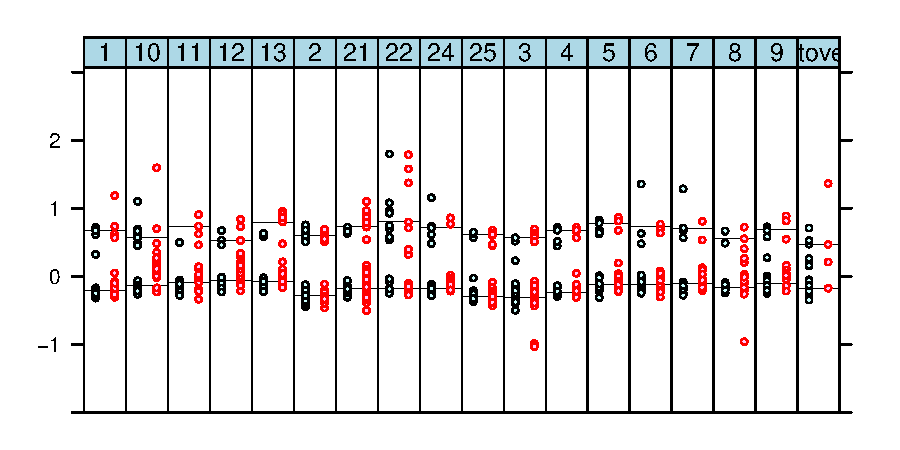
\includegraphics[scale=.5] {figures/KIR3DS1-preQC.pdf}
    \caption{ \label{Figure-S1:a}
      Pre-QC \gene{KIR3DS1} $\Delta$Ct}
    \end{subfigure}
    \begin{subfigure}[b]{.4\textwidth}
    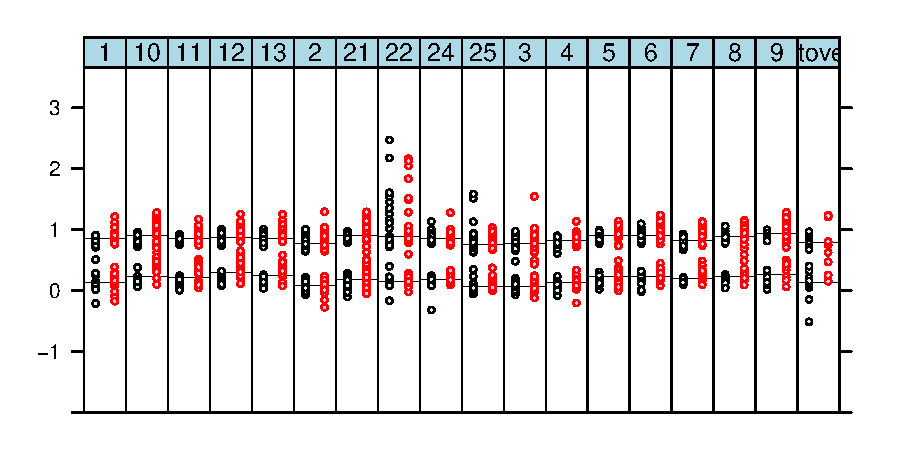
\includegraphics[scale=.5] {figures/KIR3DL1-preQC.pdf}
    \caption{ \label{Figure-S1:b}
      Pre-QC \gene{KIR3DL1} $\Delta$Ct}
    \end{subfigure}
    %
    \begin{subfigure}[b]{.4\textwidth}
    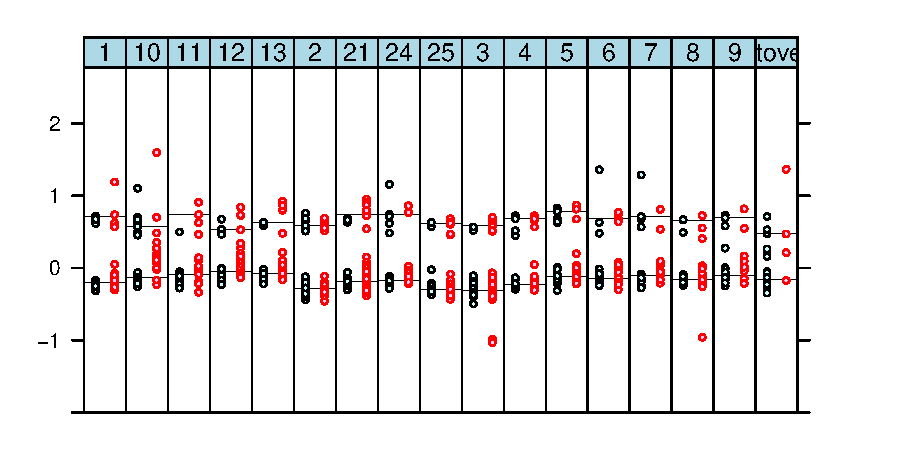
\includegraphics[scale=.5] {figures/KIR3DS1-postQC.pdf}
    \caption{Post-QC \gene{KIR3DS1} $\Delta$Ct}
    \label{}
    \end{subfigure}
    \begin{subfigure}[b]{.4\textwidth}
    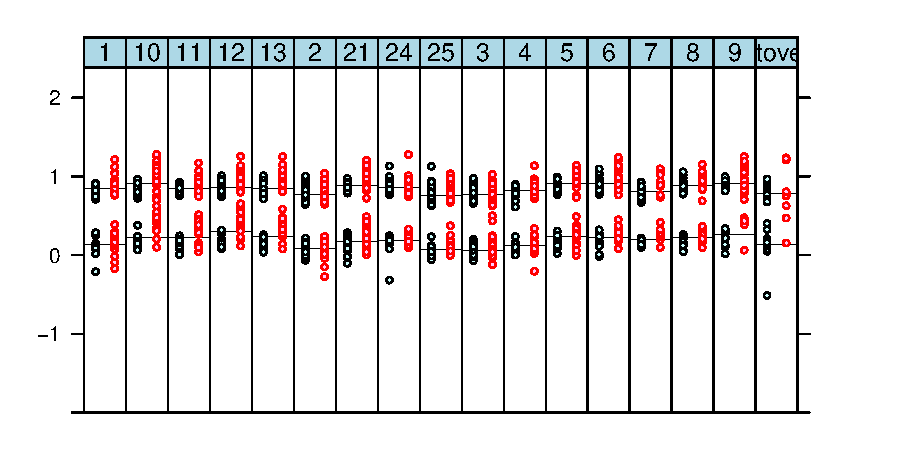
\includegraphics[scale=.5] {figures/KIR3DL1-postQC.pdf}
    \caption{Post-QC \gene{KIR3DL1} $\Delta$Ct}
    \label{}
    \end{subfigure}
    %
    \begin{subfigure}[b]{.4\textwidth}
    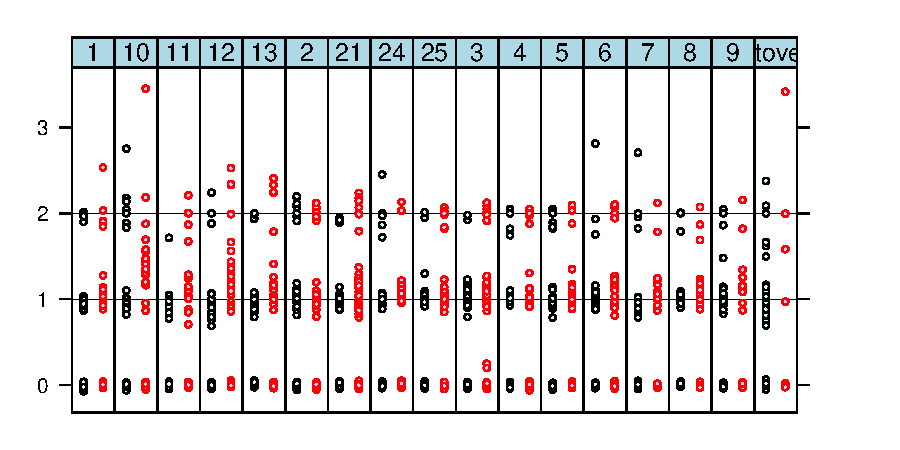
\includegraphics[scale=.5] {figures/KIR3DS1-peaknormalised.pdf}
    \caption{Peak normalised \gene{KIR3DS1} $\Delta$Ct}
    \label{}
    \end{subfigure}
    \hspace{3cm}
    \begin{subfigure}[b]{.4\textwidth}
    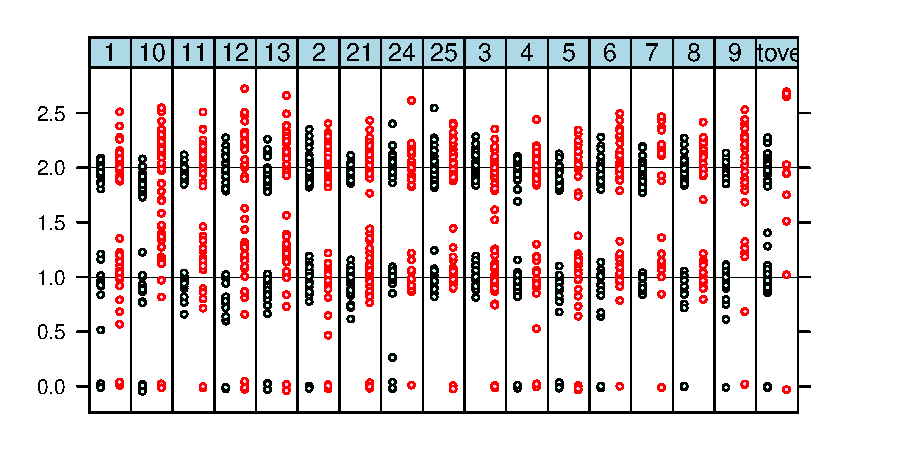
\includegraphics[scale=.5] {figures/KIR3DL1-peaknormalised.pdf}
    \caption{Peak normalised \gene{KIR3DL1} $\Delta$Ct}
    \label{Figure-S1:f}
    \end{subfigure}
    %
    \mycaption{Figure-S1}
    { \gene{KIR3DS1} and \gene{KIR3DL1} $\Delta$Ct values for cases (red) and controls (blue) per qPCR plate.  }
    {
      Plate 22 stands out as the noisiest for both \gene{KIR3DL1} (a) and \gene{KIR3DS1} (b), and so is subsequently dropped as part of the QC (c and d).
      Negative $\Delta$Ct are not displayed for pre and post QC so as to better visualise the one and two copy number groups.
      Normalisation consists a linear transform which maps the medians of the one and two copy groups from each plate to 1 and 2 (e and f).
      After normalisation, negative $\Delta$Cts values are assigned to zero.
    }
\end{figure}

\subsection{Bivariate clustering: copy number calling in qPCR data}
%\subsection{Two dimensional clustering enables accurate copy number calling in qPCR data} 


%% Figure 1
\myfigure{scale=.5}{Figure-1}
{Copy number calling of \gene{KIR3DL1}/\gene{KIR3DS1} from qPCR $\Delta$Ct.}
{ On the left, the median normalised $\Delta$Ct values for \gene{KIR3DS1} and
\gene{KIR3DL1} are shown with the results of clustering into the eight
copy number groups coloured according to the group with the
highest posterior probability.  The three most common copy number groups are the
ones with a total copy number of two: \gene{KIR3DL1} 0-2 (dark green),
\gene{KIR3DL1}/\gene{KIR3DS1} 1-1 (pink) and \gene{KIR3DS1} 2-0 (dark
blue).  The ellipses delimit the $95^{th}$ percentile.  On the right, the
counts of the most probable copy number state are shown for cases and
controls.}

Samples which yielded one or less Ct reading for Fam-KIR3DL1 or
Cy5-KIR3DS1, but all four Ct readings for the reference DFO-STAT6,
were assumed to contain zero copies of \gene{KIR3DL1} or
\gene{KIR3DS1}.  For the remainder of the samples, I called copy number groups
by fitting a mixture of bivariate Gaussian distributions to the two
dimensional normalised $\Delta$Ct values, allowing for eight
\gene{KIR3DS1}/\gene{KIR3DL1} copy number groups: three common groups of two copy
numbers (0-2, 1-1, 2-0) and five
rarer groups of lower or higher copy numbers
(\Cref{Figure-1}).  The mixture was fitted using
an \gls{EM} algorithm \citep{Young:2009ty} with initial parameters
calculated from the clusters returned by k-means with centers set to
the eight expected locations of the copy number groups.
After fitting the mixture model each sample was assigned a posterior
probability of belonging to each of the eight copy number groups which
allows for uncertainty in copy number calling.  These posterior
probabilities were taken into account in downstream statistical
analysis via multiple imputation.

Raw median $\Delta$Ct distributions varied across plates which prevented simple visual copy number assignment (\Cref{Figure-S1}).
After normalisation, samples repeated across different plates showed good reproducibility (\Cref{Figure-S3}) and two dimensional clustering enabled 1474 samples to be confidently assigned to a single copy number group, including all samples with known copy number which were assigned to the correct cluster.

%Firstly, we obtained posterior probabilities by fitting bivariate Gaussian distributions to our normalised combined KIR3DS1 and KIR3DL1 $\Delta$Ct values.
Jointly clustering on \gene{KIR3DL1} and \gene{KIR3DS1}, has the advantage of exploiting the correlation between the $\Delta$Ct values. 
For example, this can be seen in plate 10, where noisy cases (\Cref{Figure-S1}.f) are difficult to assign as one or two copies based solely on their \gene{KIR3DL1} $\Delta$Ct, but are much more clearly distinguishable when I also consider their \gene{KIR3DS1} $\Delta$Ct value (\Cref{Figure-S2}).
%For example, this can be seen in plate 10, where noisy cases (\Cref{Figure-S1}) are hard to assign as one or two copies based solely on their \gene{KIR3DL1} $\Delta$Ct, but are much more clearly distinguishable when we also consider their \gene{KIR3DS1} $\Delta$Ct value (\Cref{Figure-S2}).

%We allowed for the limited uncertainty of copy number calling by means of multiple imputation.


\begin{figure}[h]
    \centering
        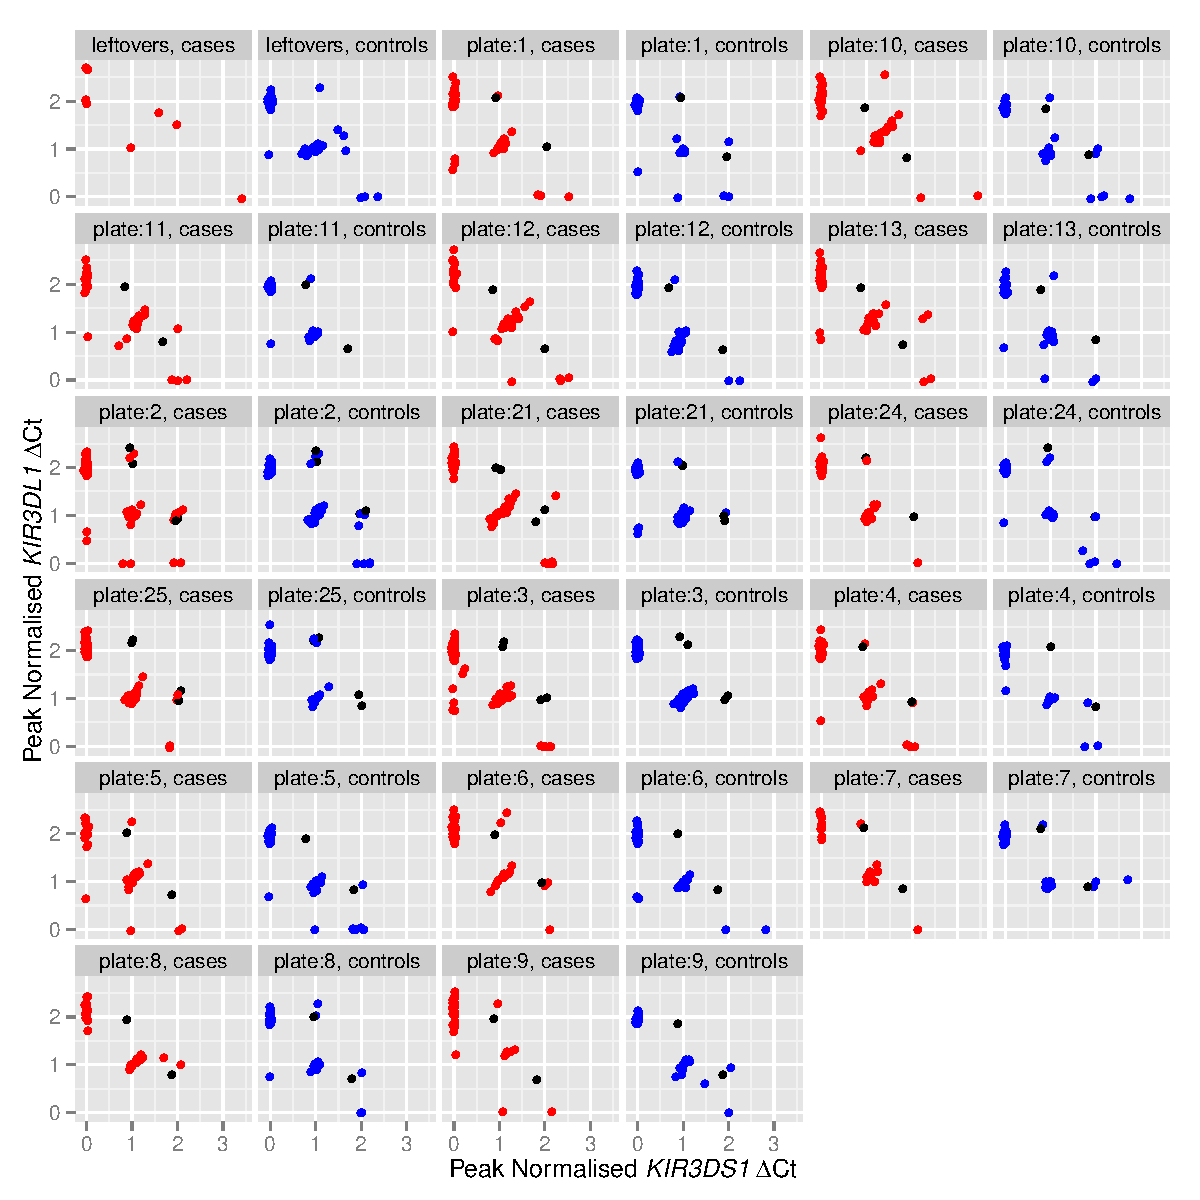
\includegraphics[scale=.9] {figures/Figure-S2.pdf}
    \mycaption{Figure-S2}
        {Post-QC cases (red) and controls (blue) are plotted separately for each qPCR plate.}
        { The samples with known \gene{KIR3DL1}/\gene{KIR3DS1} copy number are plotted in black.
        We can see that there is a larger spread in cases than in controls which is especially clear in the 1-1 copy number group.
        Also, it is apparent that the $\Delta$Ct of \gene{KIR3DL1} and \gene{KIR3DS1} are correlated in the 1-1, 2-1 and 1-2 groups.
        We exploited this correlation in the copy number calling by doing bivariate clustering.  }
\end{figure}



\begin{figure}[h]
    \centering
    \begin{subfigure}[b]{.4\textwidth}
        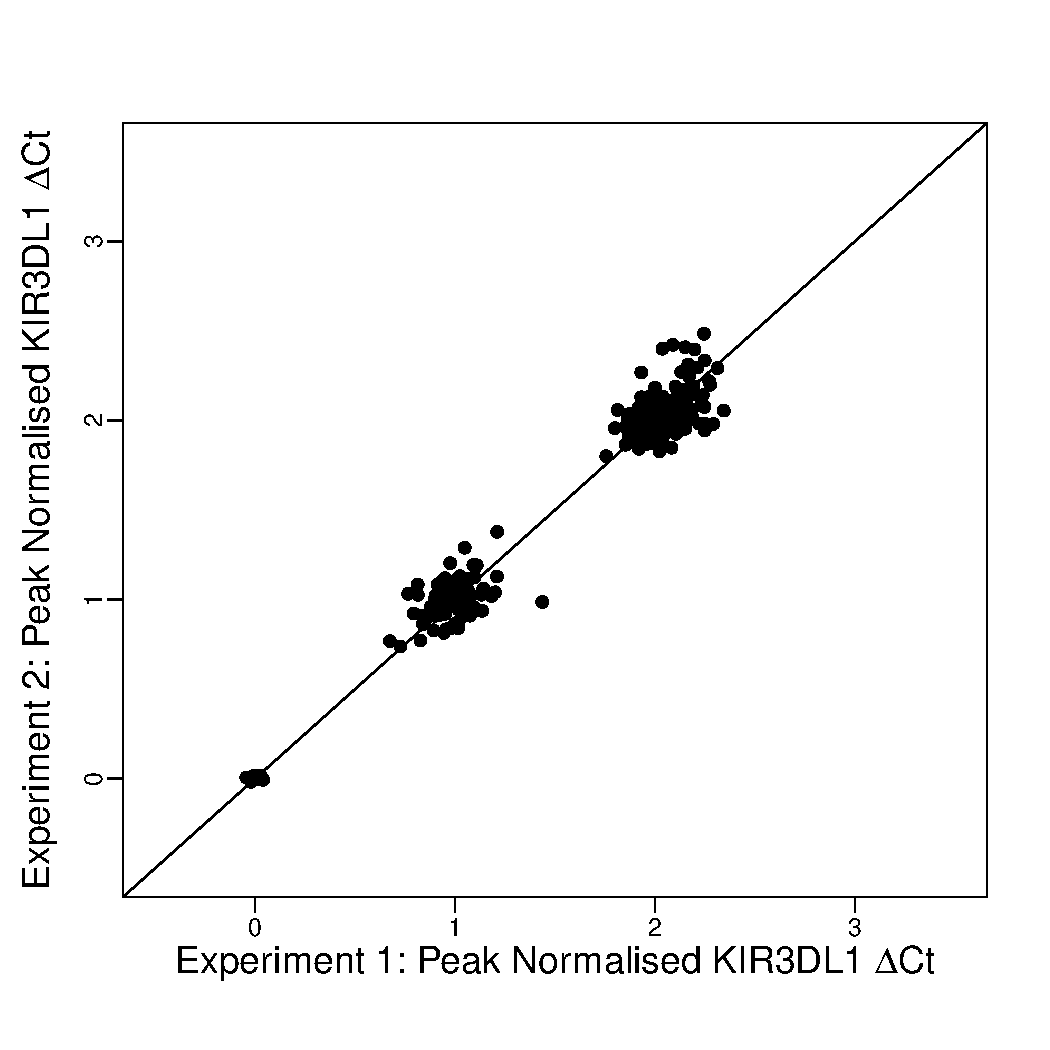
\includegraphics[scale=.4] {figures/DL1-repeatability.pdf}
        \caption{Repeatability of \gene{KIR3DL1} $\Delta$Ct post normalisation and QC ($r^{2}=0.961$).}
    \end{subfigure}
    ~
    \begin{subfigure}[b]{.4\textwidth}
        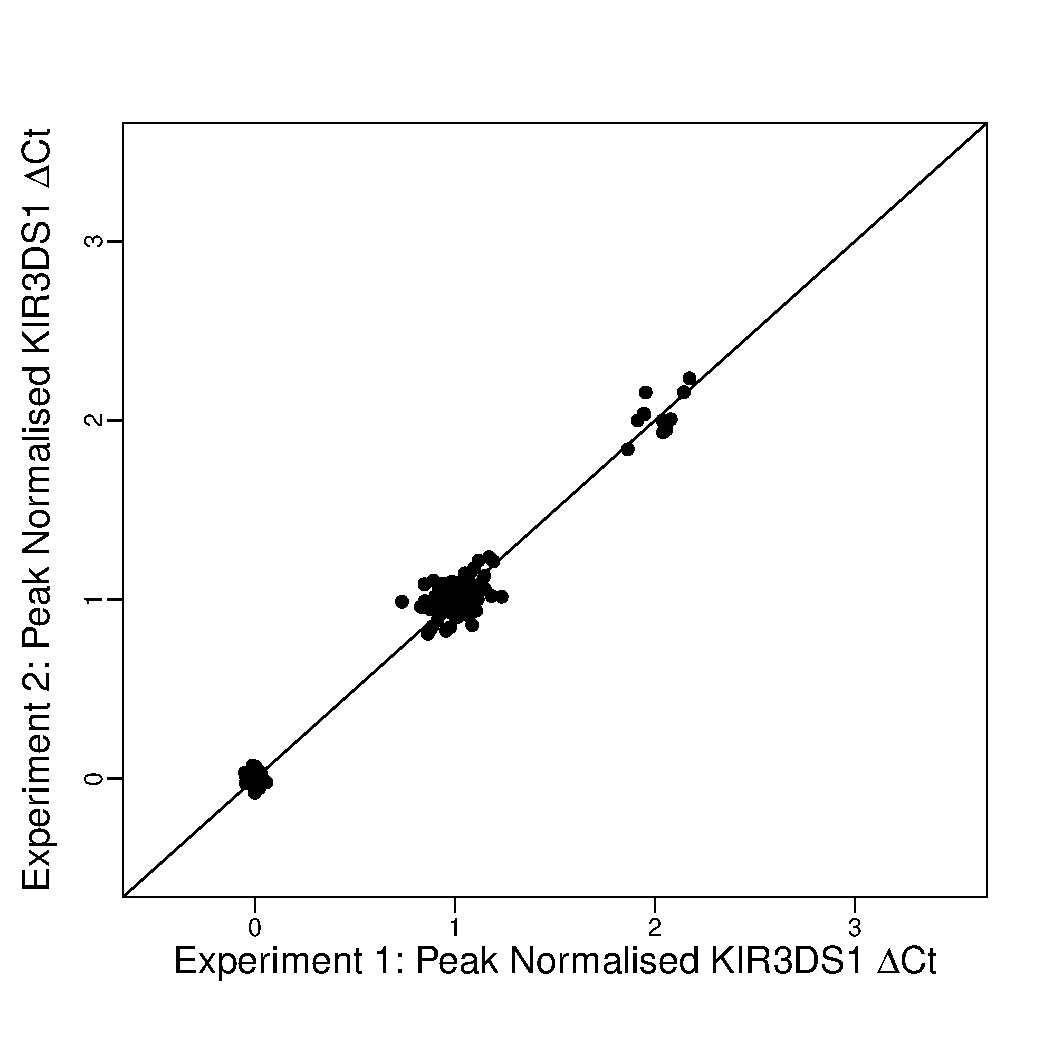
\includegraphics[scale=.4] {figures/DS1-repeatability.pdf}
        \caption{Repeatability of \gene{KIR3DS1} $\Delta$Ct post normalisation and QC ($r^{2}=0.99)$.}
        \label{}
    \end{subfigure}
    \mycaption{Figure-S3}
    {Repeatability of qPCR assay.}
    {
        In order to assess the reliability of the qPCR assay 310 samples were re-analysed.
        We found very high reproducibility of the $\Delta$Ct values ($r^{2} > 0.96)$ confirming the reliability of our qPCR assay.
        $r^2$ is the Pearson correlation squared.
        %Samples on four plates were repeated to assess 
        %The points are coloured by genotype group as defined in \Cref{figure:fuzzy-genotyping}.
        %302 samples
    }
\end{figure} 




\subsection{\gls{knn} classification: copy number imputation into the SNP data}
%\subsection{Copy number imputation into extended samples by integration of SNP array data and qPCR data} 

%% Figure 2
\begin{figure}[h!]
  \centering
  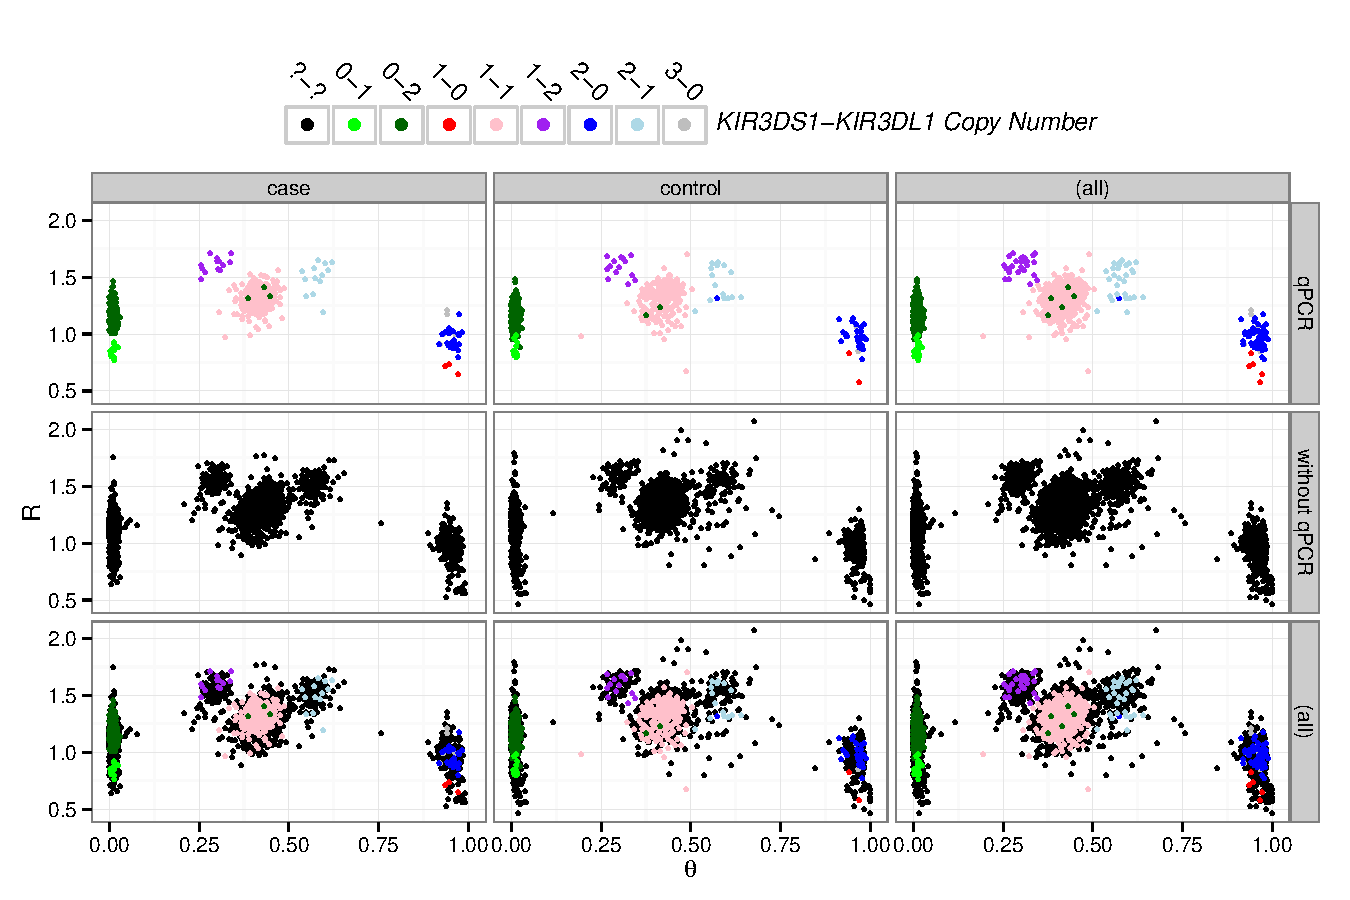
\includegraphics[scale=.5]{figures/Figure-2.pdf}
  \mycaption{Figure-2}
  {Overlay of ImmunoChip and qPCR samples for $R$ and $\theta$ at SNP rs592645.}
  { Samples are coloured by the most likely \gene{KIR3DS1}-\gene{KIR3DL1} copy number
  group according to the qPCR analysis (see \Cref{figure:Figure-1}).  The
  first and second row split the samples on the availability of qPCR data, and
  the third row is the overlay of the samples from the first and second row.
  The first and second column split the samples by case-control status and the
  third column is the overlay of the samples from the first and second column.}
\end{figure}

We extended our sample size by using the subset of samples common between the qPCR and SNP datasets, 747 cases and 727 controls, to train a k-nearest neighbour (knn) classifier to predict \gene{KIR3DL1}/\gene{KIR3DS1} copy number using the $R$ and $\theta$ signals from ImmunoChip SNPs.

Each of 30 SNPs lying within the \gene{KIR3DL1} (since \gene{KIR3DS1} is not on the reference genome) region were assessed for association with either \gene{KIR3DL1} or \gene{KIR3DS1} copy number in individual linear regression of copy number against $R$ and $\theta$ (\Cref{Table-S4}).
%Nineteen SNPs were significantly associated (\Cref{Table-S4}), with rs592645 the most strongly predictive (\Cref{Figure-2}).
SNP signals, $R$ and $\theta$, showed good association with copy numbers of \gene{KIR3DL1} and of \gene{KIR3DS1} for 19 of 30 SNPs in the \gene{KIR3DL1} region (\Cref{Table-S4}).
The best example is shown in \Cref{Figure-2}, in which seven clusters for SNP \snp{rs592645} can be discerned that correspond closely with qPCR derived
\gene{KIR3DL1}/\gene{KIR3DS1} copy numbers.
This is also visually apparent in \Cref{all-snps} where SNP \snp{rs592645} shows the best clustering of copy number out of those 30 SNPs.
\Cref{Figure-2} also illustrates a number of important points about using SNP signals for imputation.
First, $\theta$ corresponds to the ratio of copies of \gene{KIR3DL1} to \gene{KIR3DS1}, while $R$ corresponds to the total copy number.
Second, some clusters overlap; without the qPCR data, the number of clusters and their boundaries would be difficult to define, particularly along the $R$ axis.
Finally, the clusters are in slightly different positions in cases and controls, reflecting the known sensitivity of genotyping chips to subtle differences in DNA preparation and storage conditions.
This has two implications: probabilistic clustering of the SNP data alone is likely to be poor in the combined sample, while unsupervised clustering of cases and controls separately when clusters are not clearly separated risks increasing type 1 error rates \citep{Plagnol:2007dw}.
Instead, I used the qPCR copy numbers as training data to perform supervised clustering of the SNP signals.

We first explored the validity of our imputation approach by means of \gls{LOOCV} in the samples with qPCR data.
We examined using all nineteen predictive SNPs, or various subsets, and found optimal knn imputation was achieved with the single most predictive SNP,
\snp{rs592645} with $k=8$, which minimised the mean \gls{LOOCV} error rate to \pct{2.0} across ten multiply imputed qPCR datasets (\Cref{Figure-3}).  

We also explored the effect of varying the size of the training data set by setting KIR gene copy numbers to missing for a randomly chosen subset of samples and imputing them in the remaining samples.
We suggest that only 295 samples are required to achieve \gls{LOOCV} error rates $<$ \pct{5} and 590 for error rates $<$ \pct{2.5} (\Cref{Figure-4}).


\rowcolors{2}{white}{white} 
\begin{table}[h]
\begin{center}
\footnotesize
\begin{tabular}{rlrllrr}
  \hline
Name                    & Position & SNP   & GenCall QC  & p-value $\theta$  & p-value R \\
  \hline
seq-rs597598            & 60007252 & [A/G] & ok          & 3.19E-03 & 7.81E-01 \\
seq-rs598452            & 60007428 & [A/G] & ok          & 6.53E-01 & 2.62E-01 \\
\rowcolor{LightCyan}
seq-t1d-19-60007809-C-G & 60007809 & [G/C] & ok          & 3.64E-02 & 6.27E-06 \\
seq-rs55761930          & 60008141 & [T/C] & ok          & 6.33E-01 & 6.12E-01 \\
\rowcolor{LightCyan}
seq-rs10500318          & 60012591 & [A/G] & ok          & 7.59E-11 & 1.31E-13 \\
\rowcolor{LightRed}
seq-rs592645            & 60012739 & [A/T] & ok          & 8.85E-01 & 3.38E-09 \\
seq-rs604077            & 60013208 & [A/G] & ok          & 4.82E-03 & 1.20E-01 \\
\rowcolor{LightCyan}
seq-rs604999            & 60013409 & [A/G] & ok          & 1.77E-15 & 9.99E-04 \\
\rowcolor{LightCyan}
seq-t1d-19-60014013-A-C & 60014013 & [T/G] & lowcallrate & 8.74E-01 & 3.15E-08 \\
\rowcolor{LightCyan}
rs3865507               & 60014188 & [T/G] & ok          & 8.62E-03 & 6.93E-17 \\
\rowcolor{LightCyan}
seq-rs3865510           & 60016051 & [A/C] & ok          & 2.23E-10 & 2.04E-10 \\
seq-rs648689            & 60016286 & [A/G] & ok          & 2.31E-01 & 1.03E-02 \\
\rowcolor{LightCyan}
seq-rs649216            & 60016447 & [T/C] & ok          & 2.85E-02 & 1.04E-13 \\
\rowcolor{LightCyan}
rs581623                & 60018551 & [A/G] & ok          & 3.76E-02 & 2.06E-13 \\
\rowcolor{LightCyan}
seq-rs4806568           & 60022568 & [A/G] & lowcallrate & 1.44E-20 & 2.93E-01 \\
seq-rs674268            & 60024002 & [T/C] & lowcallrate & 1.43E-02 & 2.90E-01 \\
rs12461010              & 60024413 & [A/G] & ok          & 4.72E-01 & 1.72E-01 \\
\rowcolor{LightCyan}
seq-rs2295805           & 60028513 & [T/C] & lowcallrate & 9.55E-08 & 8.40E-04 \\
seq-rs12976350          & 60030391 & [T/C] & lowcallrate & 1.70E-05 & 5.07E-01 \\
seq-t1d-19-60034052-C-T & 60034052 & [A/G] & hwe         & 3.27E-02 & 4.07E-01 \\
\rowcolor{LightCyan}
rs4806585               & 60038236 & [T/G] & hwe         & 2.20E-11 & 2.42E-02 \\
\rowcolor{LightCyan}
seq-rs62122181          & 60039178 & [T/C] & lowcallrate & 2.40E-13 & 2.26E-01 \\
rs10422740              & 60052298 & [T/C] & monomorph   & 7.78E-01 & 8.49E-02 \\
\rowcolor{LightCyan}
rs640345                & 60054671 & [A/G] & ok          & 3.61E-07 & 6.83E-02 \\
seq-t1d-19-60054973-T-C & 60054973 & [A/G] & ok          & 2.92E-01 & 2.28E-04 \\
\rowcolor{LightCyan}
seq-t1d-19-60056605-A-T & 60056605 & [A/T] & ok          & 3.99E-01 & 1.48E-16 \\
\rowcolor{LightCyan}
seq-t1d-19-60056721-C-T & 60056721 & [A/G] & ok          & 9.02E-01 & 2.04E-09 \\
\rowcolor{LightCyan}
seq-rs10407958          & 60063974 & [T/A] & ok          & 1.06E-02 & 5.45E-10 \\
\rowcolor{LightCyan}
seq-rs1654644           & 60065174 & [T/G] & ok          & 7.94E-14 & 5.21E-12 \\
\rowcolor{LightCyan}
rs3826878               & 60069023 & [A/G] & ok          & 2.63E-05 & 3.55E-06 \\
   \hline
\end{tabular}
%xtable(kir, display=c('d','s','d','s','s','E','E')) 
\end{center}
    \mycaption{Table-S4}
    {ImmunoChip SNPs which fall in \gene{KIR3DL1}.}
    {
    The 30 ImmunoChip SNPs which fall in the \gene{KIR3DL1} region according to build36/hg18, nineteen of which
    are significantly associated with \gene{KIR3DL1}/\gene{KIR3DS1} copy number (highlighted in blue).
    \gene{KIR3DS1} is missing from build36/h18.
    SNP \snp{rs592645} which has shown to be highly predictive of \gene{KIR3DL1}/\gene{KIR3DS1} copy number is
    highlighted in light red.
    The QC column reports the GenCall quality control diagnosis: ok, low call rate, failure to meet Hardy Weinberg equilibrium (hwe) or
    monomorphic SNP.
% GenCall Score:
%http://res.illumina.com/documents/products/technotes/technote_gencall_data_analysis_software.pdf
        %http://www.biomedcentral.com/1471-2105/12/68
    }
\end{table}


%% Figure 
\begin{figure}
\centering
  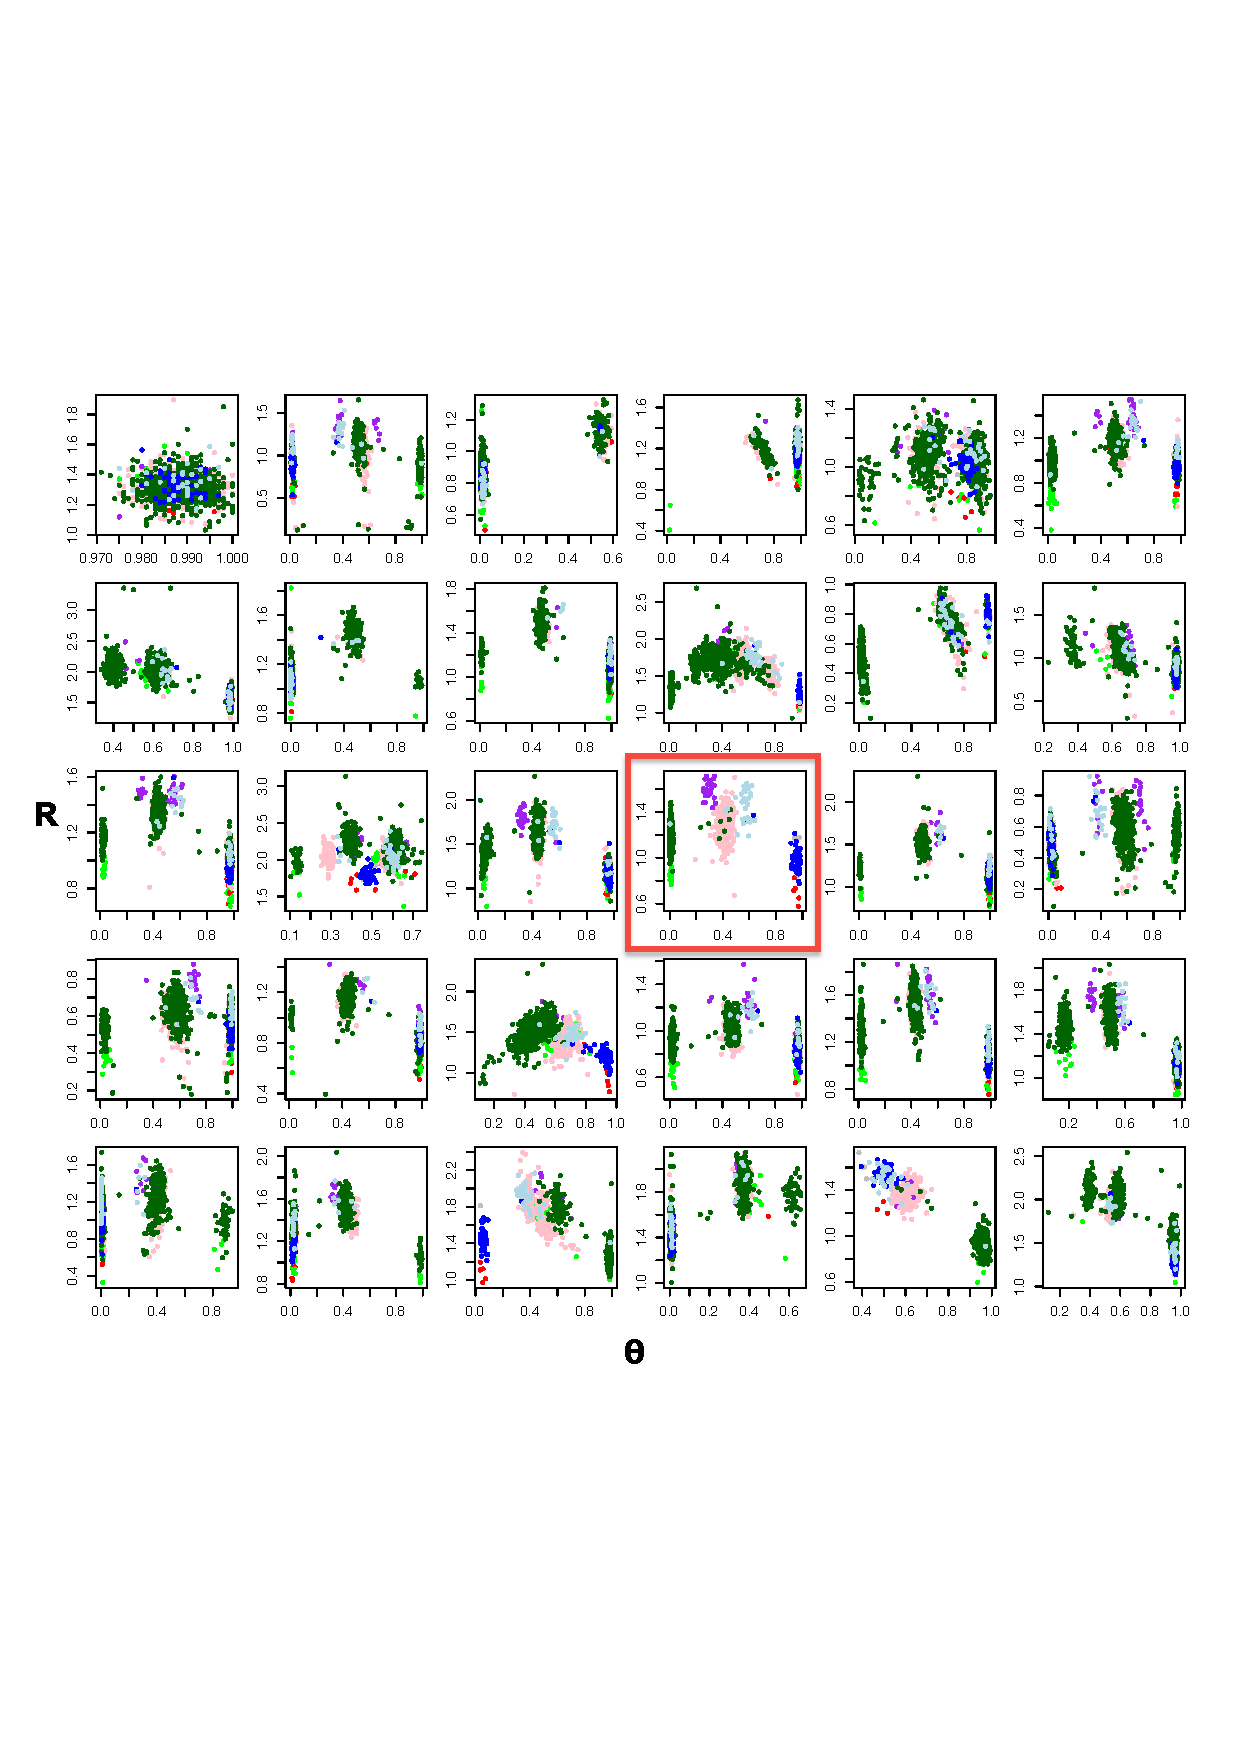
\includegraphics[scale=.8]{figures/all-snps.pdf}
  \mycaption{all-snps}
  {Signal plots of ImmunoChip SNPs which fall in the \gene{KIR3DL1} region.}
  { Each of the 30 ImmunoChip SNPs from \Cref{Table-S4}, coloured by \gene{KIR3DL1}/\gene{KIR3DS1} copy number (see \Cref{Figure-2} for legend).
  SNP \snp{rs592645} (red square) shows the best clustering by copy number.  }
\end{figure}




%% Figure 3
\begin{figure}[h!]
  \centering
  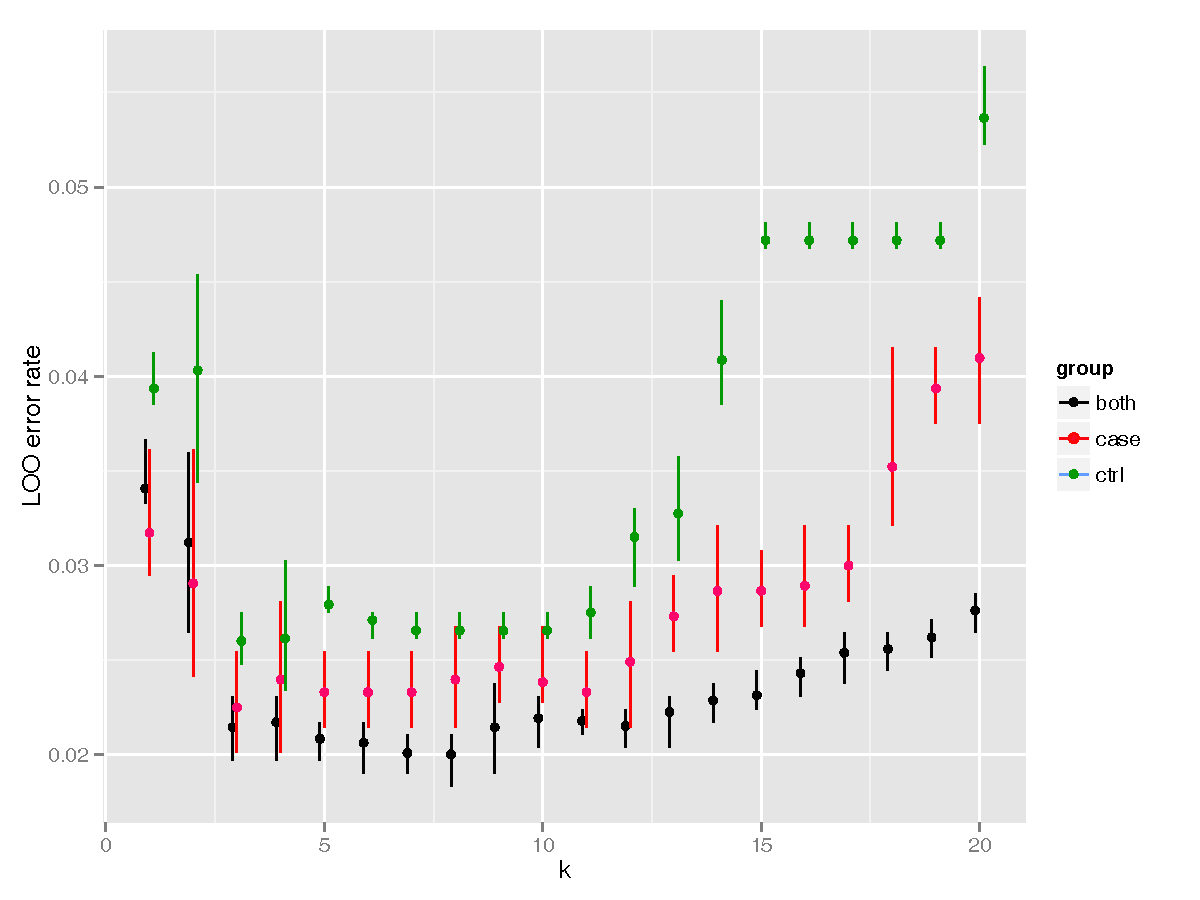
\includegraphics[scale=.5]{figures/Figure-3.pdf}
  \mycaption{Figure-3}
  {Leave-one-out crossvalidation error rate for k-nearest neighbour (KNN) prediction.}
  {
  Leave-one-out cross validation error rates
  obtained from \gls{knn} prediction
  of \gene{KIR3DL1}/\gene{KIR3DS1} copy numbers from the $R$ and $\theta$ signals of SNP \snp{rs592645}.
  Each point shows the proportion of samples for which the knn predicted copy number did not 
  match the qPCR call, averaged over ten multiply imputed qPCR call datasets
  (using the posterior probabilities from \Cref{Figure-1}). 
  Error bars show the minimum and maximum error rates over the ten multiply imputed datasets.
  Knn was run in parallel for cases only, controls only and on all samples together.
  The minimum error rate is achieved for $k=8$ when the prediction uses both cases and controls.}
\end{figure}

%% Figure 4
\begin{figure}[h!]
  \centering
  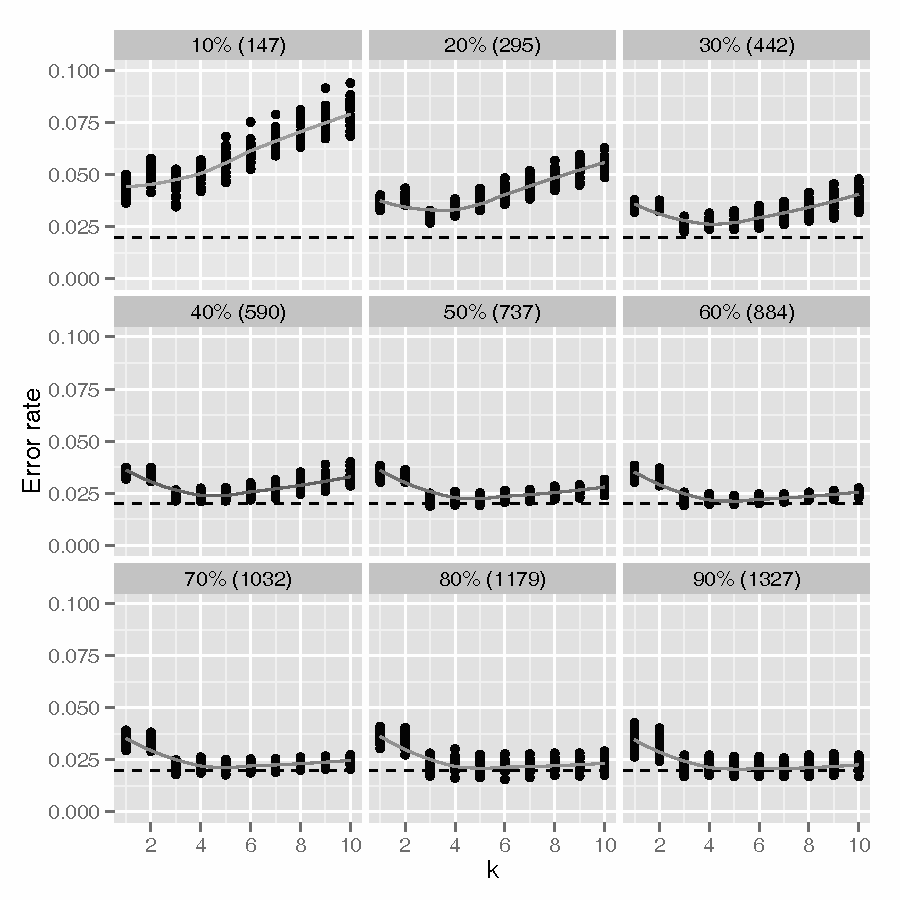
\includegraphics[scale=.5]{figures/Figure-4.pdf}
  \mycaption{Figure-4}
  {Error rate of k-nearest neighbour prediction from $R$ and $\theta$ of SNP \snp{rs592645} in random subset of samples.}
  { Each panel shows the LOOCV error rates of \gene{KIR3DL1}/\gene{KIR3DS1} copy number prediction
  from $R$ and $\theta$ of \snp{rs592645} in the remaining unlabeled samples
  when using a different size subset of the training data.
  The percentage of the complete training data set and the size of the subset is given in the title of each panel.
  Each point represents the LOOCV error rate averaged over ten multiply imputed qPCR call datasets
  (using the posterior probabilities from \Cref{Figure-1}). 
  Smoothing lines show the average over 25 independent random subsets of training data.
  The black dashed line represent the observed error rate in the complete sample.
  As the size of the training dataset increases the error rate becomes less sensitive to the choice of the parameter k.
  Only 295 samples are required to achieve LOOCV error rates $<5\%$ and 590 for error rates $<2.5\%$. }
\end{figure}

\section{Association testing of \emph{KIR3DL1}/\emph{KIR3DS1} copy number with T1D}

In calling copy number states from qPCR data, rare amplifications of three or more copies are harder to classify with certainty than more common copy number states such as zero, one, or two copies.
This is mainly because copy numbers higher than two are rare but also because the $\Delta$Ct difference between successive higher copy numbers shrinks logarithmically.
However dropping samples which can not be classified with certainty can lead to bias.
A less biased approach is to allow for uncertainty by using posterior probabilities in the association tests \citep{Plagnol:2007dw}.  

%We implemented this approach by using the posterior probabilities from the model based clustering, followed by logistic regression on multiply imputed data in order to estimate the effect size and variance of the regression coefficients.  
%in a regression on incomplete data sets.
%The effect is to increase the variance of the estimates 
%Secondly, using the posterior probabilities, we did multiple imputation through simulation, thus estimating the effect size and variance of coefficients in the logistic regression against T1D status.

We tested for association of T1D with the predicted copy numbers from the qPCR and SNP datasets using logistic regression.
We allowed for uncertainty in the copy number call when estimating individual odds ratios by using ten multiply imputed datasets \citep{Cordell:2006da},
and averaging results over those using the \Rpackage{mitools}.

We allowed for statistical interaction with HLA-Bw4 by repeating the association test in the subsets of carriers of the target ligand HLA-Bw4 epitopes, HLA-Bw4 for \gene{KIR3DL1} and the putative ligand HLA-Bw4-80I for \gene{KIR3DS1}.
We directly tested for interaction with a more powerful case-only $\chi^2$ test \citep{Yang:1999wk,Cordell:2009jb}.


Finally, I attempted to correlate \gene{KIR3DL1}/\gene{KIR3DS1} copy number with T1D status.
We performed an \Gls{ANOVA} $\chi^{2}_{7}$ test on the logistic model using the most likely copy number group,
which yielded a p-value of $0.9776$ in the qPCR and $0.1739$ in the SNP dataset, thus showing no overall association.
We also used multiple imputation to assess the effect of individual copy number groups while allowing for the uncertainty in copy number calling.
We found no significant evidence for association, in the qPCR
data (747 cases and 727 controls) nor in the extended SNP data (6744
cases and 5362 controls) (\Cref{Table-1}).
By expanding to these large samples, which would be infeasible to genotype directly with
qPCR, I am able to exclude odds ratios outside of the range
[.92; 1.08] for the common copy number groups with \pct{95} certainty.

We also repeated the association tests in the  subset of individuals
carriers of the HLA-Bw4 epitope, and again detected no significant
association  (\Cref{Table-2}).
A disadvantage of subsetting by HLA-Bw4 is that power is lost by greatly reducing the sample size. 
A more powerful test for interaction between unlinked genes is a case-only test \citep{Yang:1999wk}.
If there were an interaction effect between \gene{KIR3DL1}/\gene{KIR3DS1} and HLA-Bw4 then this should be detectable
as a difference in \gene{KIR3DL1}/\gene{KIR3DS1} copy number frequencies across HLA-Bw4 strata in the cases.
However, I found no significant difference in either the qPCR or SNP data sets,
before or after reducing the degrees of freedom by collapsing the KIR copy number to present/absent to
increase power (\Cref{Table-3}). 

%% Table 1
\begin{table}[h]
\hspace{-2cm}
\footnotesize
\begin{tabularx}{\textwidth}{ccrrrr|crrrr}
%% Table 1.a
  \mc{1}{l}{\textbf{a)}} & \mc{5}{c}{qPCR} & \mc{5}{c}{SNP} \\
  \rowcolor{Gray}
  \gene{KIR3DS1}-\gene{KIR3DL1} & case:control & total & OR   & 95\%CI    & p-value & case:control & total & OR   & 95\%CI    & p-value \\
  \cc{0-2}               & 444:446      & 890   & 1.00 &           &         & 4094:3222    & 7316  & 1    &           & \\
  \cc{1-1}               & 229:207      & 436   & 1.11 & 0.88-1.40 & 0.3673  & 2050:1628    & 3678  & 0.99 & 0.92-1.07 & 0.8349 \\
  \cc{2-0}               & 26:28        & 54    & 0.92 & 0.52-1.61 & 0.7713  & 229:225      & 454   & 0.79 & 0.65-0.96 & 0.0193 \\
  \cc{2-1}               & 15:16        & 31    & 0.94 & 0.46-1.93 & 0.8695  & 121:101      & 222   & 0.92 & 0.7-1.2   & 0.5246 \\
  \cc{1-2}               & 13:14        & 27    & 0.93 & 0.43-2.01 & 0.8587  & 98:74        & 172   & 1.04 & 0.77-1.42 & 0.7822 \\
  \cc{0-1}               & 13:11        & 24    & 1.19 & 0.53-2.68 & 0.6794  & 116:77       & 193   & 1.19 & 0.89-1.59 & 0.2535 \\
  \cc{1-0}               & 4:3          & 7     & 1.34 & 0.30-6.02 & 0.7031  & 25:21        & 46    & 0.94 & 0.52-1.68 & 0.8255 \\
  \cc{3-0}               & 3:2          & 5     & 1.52 & 0.27-8.62 & 0.6369  & 11:14        & 25    & 0.74 & 0.3-1.82  & 0.518 \\
  \cmidrule(l{5pt}r{5pt}){2-3} \cmidrule(l{5pt}r{5pt}){6-6} \cmidrule(l{5pt}r{5pt}) {7-8} \cmidrule(l{5pt}r{5pt}){11-11}
  \mcc{Overall} & \mcc{747:727} & \mcc{1474} &  \mcc{} &  \mcc{} &  \mcc{0.9842} & \mcc{6744:5362} & \mcc{12106}  &  \mcc{} & \mcc{} &  \mcc{0.3552} \\
 \\
%% Table 1.b
  \mc{1}{l}{\textbf{b)}} & \mc{5}{c}{qPCR} & \mc{5}{c}{SNP} \\
  \rowcolor{Gray}
  \gene{KIR3DL1} & case:control & total & OR   & 95\%CI    & p-value & case:control & total & OR   & 95\%CI    & p-value \\
  \cc{2}         & 457:460      & 917   & 1.00 &           &         & 4192:3296    & 7488  & 1    &           & \\
  \cc{1}         & 257:234      & 491   & 1.11 & 0.89-1.38 & 0.3702  & 2287:1806    & 4093  & 0.99 & 0.92-1.07 & 0.8883 \\
  \cc{0}         & 33:33        & 66    & 1.01 & 0.61-1.66 & 0.9795  & 265:260      & 525   & 0.8  & 0.67-0.96 & 0.0151 \\
  \cmidrule(l{5pt}r{5pt}){2-3} \cmidrule(l{5pt}r{5pt}){6-6} \cmidrule(l{5pt}r{5pt}) {7-8} \cmidrule(l{5pt}r{5pt}){11-11}
  \mcc{Overall} & \mcc{747:727} & \mcc{1474} &  \mcc{} &  \mcc{} &  \mcc{0.6651} & \mcc{6744:5362} & \mcc{12106}  &  \mcc{} & \mcc{} &  \mcc{0.0506} \\
 \\
 \\
%% Table 1.c
  \mc{1}{l}{\textbf{c)}} & \mc{5}{c}{qPCR} & \mc{5}{c}{SNP} \\
  \rowcolor{Gray}
  \gene{KIR3DS1} & case:control & total & OR   & 95\%CI    & p-value & case:control & total & OR   & 95\%CI    & p-value \\
  \cc{0}         & 457:457      & 914   & 1.00 &           &         & 4210:3299    & 7509  & 1    &           & \\
  \cc{1}         & 246:224      & 470   & 1.10 & 0.88-1.37 & 0.4096  & 2173:1723    & 3896  & 0.99 & 0.91-1.07 & 0.7785 \\
  \cc{2}         & 41:44        & 85    & 0.94 & 0.60-1.47 & 0.7787  & 350:326      & 676   & 0.83 & 0.71-0.97 & 0.0212 \\
  \cc{3}         & 3:2          & 5     & 1.24 & 0.21-7.28 & 0.8084  & 11:14        & 25    & 0.74 & 0.3-1.82  & 0.5119 \\
  \cmidrule(l{5pt}r{5pt}){2-3} \cmidrule(l{5pt}r{5pt}){6-6} \cmidrule(l{5pt}r{5pt}) {7-8} \cmidrule(l{5pt}r{5pt}){11-11}
  \mcc{Overall} & \mcc{747:727} & \mcc{1474} &  \mcc{} &  \mcc{} &  \mcc{0.8044} & \mcc{6744:5362} & \mcc{12106}  &  \mcc{} & \mcc{} &  \mcc{0.1494} \\
\end{tabularx}
\mycaption{Table-1}
{Association test of \gene{KIR3DS1}-\gene{KIR3DL1} copy number with T1D.}
{
  Association with T1D tested for the joint
  \gene{KIR3DS1}-\gene{KIR3DL1} \textbf{(a)}, marginal \gene{KIR3DL1}
  \textbf{(b)} and \gene{KIR3DS1} \textbf{(c)} copy number group.
  No evidence of a significant, joint or marginal, effect detected in the
  qPCR dataset, 747 cases and 727 controls, nor in the SNP dataset, 6744 cases and 5362 controls.
  Case-control counts shown are derived from the most likely copy number assignment across the 10 multiply imputed qPCR and SNP datasets.
  Statistical inference for association is derived from the multiply imputed datasets using the \Rpackage{mitools}.
  The last row of each table contains the pooled p-value for each association test using the \Rpackage{mice}.
}
\end{table}


%% Table 2
\begin{table}[h]
\hspace{-2cm}
\footnotesize
\begin{tabularx}{\textwidth}{ccrrrr|crrrr}
  %a)
  \mc{1}{l}{\textbf{a)} HLA-Bw4 subset} & \mc{5}{c}{qPCR} & \mc{5}{c}{SNP} \\
  \rowcolor{Gray}
  \gene{KIR3DS1}-\gene{KIR3DL1} & case:control & total & OR   & 95\%CI     & p-value & case:control & total & OR   & 95\%CI     & p-value \\
  \cc{0-2}     & 259:286      & 545   & 1.00 &            &         & 1025:1156    & 2181  & 1.00 &            & \\
  \cc{1-1}     & 123:128      & 251   & 1.06 & 0.79-1.43  & 0.6976  & 556:583      & 1139  & 1.08 & 0.93-1.24  & 0.3194 \\
  \cc{2-0}     & 16:15        & 31    & 1.22 & 0.58-2.57  & 0.5985  & 61:87        & 148   & 0.79 & 0.56-1.11  & 0.1733 \\
  \cc{2-1}     & 7:13         & 20    & 0.59 & 0.23-1.51  & 0.2754  & 32:40        & 72    & 0.90 & 0.56-1.45  & 0.6695 \\
  \cc{1-2}     & 8:8          & 16    & 1.10 & 0.41-2.98  & 0.8450  & 27:32        & 59    & 0.95 & 0.57-1.60  & 0.8513 \\
  \cc{0-1}     & 10:7         & 17    & 1.58 & 0.59-4.20  & 0.3621  & 36:26        & 62    & 1.56 & 0.94-2.60  & 0.0876 \\
  \cc{1-0}     & 2:1          & 3     & 2.21 & 0.20-24.50 & 0.5187  & 7:3          & 10    & 2.63 & 0.68-10.19 & 0.1614 \\
  \cc{3-0}     & 3:0          & 3     &      &            &         & 3:1          & 4     & 3.38 & 0.35-32.51 & 0.2910 \\
  \cmidrule(l{5pt}r{5pt}) {2-3} \cmidrule(l{5pt}r{5pt}) {7-8}
  \mcc{} & \mcc{428:458} & \mcc{886} & \mcc{} & \mcc{} & \mcc{} & \mcc{1747:1928} & \mcc{3675} & \mcc{} & \mcc{} & \mcc{} \\
  \\
  %b)
  \mc{1}{l}{\textbf{b)} HLA-Bw4 subset} & \mc{5}{c}{qPCR} & \mc{5}{c}{SNP} \\
  \rowcolor{Gray}
  \gene{KIR3DL1} & case:control & total & OR   & 95\%CI    & p-value & case:control & total & OR   & 95\%CI    & p-value \\
  \cc{2}         & 267:294      & 561   & 1.00 &           &         & 1052:1188    & 2240  & 1.00 &           & \\
  \cc{1}         & 140:148      & 288   & 1.04 & 0.78-1.38 & 0.7787  & 624:649      & 1273  & 1.09 & 0.95-1.25 & 0.2414 \\
  \cc{0}         & 21:16        & 37    & 1.45 & 0.74-2.83 & 0.2822  & 71:91        & 162   & 0.88 & 0.64-1.21 & 0.4399 \\
  \cmidrule(l{5pt}r{5pt}) {2-3} \cmidrule(l{5pt}r{5pt}) {7-8}
  \mcc{} & \mcc{428:458} & \mcc{886} &  \mcc{} &  \mcc{} &  \mcc{} & \mcc{1747:1928} & \mcc{3675}  &  \mcc{} & \mcc{} &  \mcc{} \\
  \\
  %c)
  \mc{1}{l}{\textbf{c)} HLA-Bw4-80I subset} & \mc{5}{c}{qPCR} & \mc{5}{c}{SNP} \\
  \rowcolor{Gray}
  \gene{KIR3DS1} & case:control & total & OR   & 95\%CI    & p-value & case:control & total & OR   & 95\%CI    & p-value \\
  \cc{0}         & 159:187      & 346   & 1.00 &           &         & 650:734      & 1384  & 1.00 &           & \\
  \cc{1}         & 93:83        & 176   & 1.32 & 0.92-1.90 & 0.1370  & 384:365      & 749   & 1.19 & 0.99-1.42 & 0.0578 \\
  \cc{2}         & 12:14        & 26    & 1.01 & 0.45-2.24 & 0.9842  & 61:75        & 136   & 0.92 & 0.64-1.31 & 0.6376 \\
  \cc{3}         & 2:0          & 2     &      &           &         & 1:0          & 1     &      &           & \\
  \cmidrule(l{5pt}r{5pt}) {2-3} \cmidrule(l{5pt}r{5pt}) {7-8}
  \mcc{} & \mcc{266:284} & \mcc{550} &  \mcc{} &  \mcc{} &  \mcc{} & \mcc{1096:1174} & \mcc{2270}  &  \mcc{} & \mcc{} &  \mcc{} \\
  \end{tabularx}
\mycaption{Table-2} {Association test of \gene{KIR3DS1}-\gene{KIR3DL1} copy number with T1D, conditional on HLA-Bw4.}
{
In order to test whether \gene{KIR3DL1}/\gene{KIR3DS1} is associated with T1D risk conditional on the presence of the respective the HLA-Bw4 epitope,
association with T1D is tested in the subset of individuals carriers of an HLA-Bw4 epitope
for the joint \gene{KIR3DS1}/\gene{KIR3DL1} \textbf{(a)} and  marginal \gene{KIR3DL1} \textbf{(b)} copy number groups
and, also tested in the subset of individuals carriers of HLA-Bw4-80I 
for the marginal \gene{KIR3DS1} \textbf{(c)} copy number group.  
}
\end{table}


%% Table 3
\begin{table}[h]
%\hspace{-2cm}
\footnotesize
\begin{tabularx}{\textwidth}{ llrr|rr}
  \mc{2}{l}{\textbf{a)}} & \mc{2}{c}{qPCR} & \mc{2}{c}{SNP} \\
                         &                        & \cc{HLA-Bw4\texttt{-}} & \cc{HLA-Bw4\texttt{+}} & \cc{HLA-Bw4\texttt{-}} & \cc{HLA-Bw4\texttt{+}} \\
  \cc{KIR3DS1\texttt{-}} & \cc{KIR3DL1\texttt{+}} & 183                    & 269                    & 739                   & 1063 \\
  \cc{KIR3DS1\texttt{+}} & \cc{KIR3DL1\texttt{-}} & 12                     & 21                     & 40                    & 71 \\
  \cc{KIR3DS1\texttt{+}} & \cc{KIR3DL1\texttt{+}} & 113                    & 138                    & 396                   & 613 \\
  \cmidrule(l{5pt}r{5pt}) {3-4} \cmidrule(l{5pt}r{5pt}) {5-6}
  \mcc{} & \mcc{} & \mcc{} & \mcc{p-value $= 0.4094$} & \mcc{} & \mcc{p-value $= 0.4235$} \\
  \\
  \mc{2}{l}{\textbf{b)}} & \mc{2}{c}{qPCR} & \mc{2}{c}{SNP} \\
                                    &     & \cc{HLA-Bw4\texttt{-}} & \cc{HLA-Bw4\texttt{+}} & \cc{HLA-Bw4\texttt{-}} & \cc{HLA-Bw4\texttt{+}} \\
  \mc{2}{c}{\cc{KIR3DL1\texttt{-}}} & 12  & 21                      & 40          & 71 \\
  \mc{2}{c}{\cc{KIR3DL1\texttt{+}}} & 296 & 407                     & 1135         & 1676 \\
  \cmidrule(l{5pt}r{5pt}) {3-4} \cmidrule(l{5pt}r{5pt}) {5-6}
  \mcc{}                            &  \mcc{} & \mcc{} & \mcc{p-value $= 0.5144$} & \mcc{} & \mcc{p-value $= 0.3609$} \\
  \\
  \mc{2}{l}{\textbf{c)}} & \mc{2}{c}{qPCR} & \mc{2}{c}{SNP} \\
                                      &        & \cc{HLA-Bw4-80I\texttt{-}}   & \cc{HLA-Bw4-80I\texttt{+}} & \cc{HLA-Bw4-80I\texttt{-}}    & \cc{HLA-Bw4-80I\texttt{+}} \\
  \mc{2}{c}{\cc{KIR3DS1\texttt{-}}}   & 293    & 159                          & 1153                       & 649 \\
  \mc{2}{c}{\cc{KIR3DS1\texttt{+}}}   & 159    & 107                          & 673                       & 447 \\
  \cmidrule(l{5pt}r{5pt}) {3-4} \cmidrule(l{5pt}r{5pt}) {5-6}
  \mcc{}                              & \mcc{} & \mcc{} & \mcc{p-value $= 0.4922$}         & \mcc{} & \mcc{p-value $= 0.0353$} \\
\end{tabularx}
\mycaption{Table-3}
{
Case-only $\chi^{2}$ test for interaction between \gene{KIR3DS1}-\gene{KIR3DL1} copy number
and HLA-Bw4, across the ten multiply imputed qPCR and SNP datasets. 
}
{
Counts in each contingency table are derived from the most likely copy number assignment
across the multiply imputed datasets. To reduce the degrees of freedom and
improve power, I summarise copy numbers higher or equal to one by presence
(\texttt{+}) and zero by absence (\texttt{-}).  The pooled p-value of each
$\chi^{2}$ test, across the multiply imputed datasets, is given in the last row
of each contingency table. We find no significant association with HLA-Bw4,
within cases, in either the joint \textbf{(a)} or the marginal
\textbf{(b)}\textbf{(c)} \gene{KIR3DS1}-\gene{KIR3DL1} distributions.
}
\end{table}


\section{ Discussion }

\subsection{Previous association studies of KIR genes with T1D}

So far, case-control studies using PCR in different ethnicities have looked at whether the presence or absence of KIR genes but not the copy number are associated with T1D 
\citep{vanderSlik:2003gq,vanderSlik:2007hi,NikitinaZake:2004jv,Santin:2006hh,Middleton:2006ba,PARK:2006km,Mogami:2007gj,Shastry:2008id,Jobim:2010,Zhi:2011kl}.
These, however, represent an incomplete version of the KIR genotype because, as shown by \citet{Jiang:2012cf}, a considerable portion of the diversity in the KIR haplotypes arises from copy number variation.
Although presence/absence might have a stronger effect than copy number variation.
%Whether KIR is implicated in T1D is still very much a matter of debate.

%independent KIR effect
From the studies I know of, as summarised in \Cref{table:kir-t1d-studies,table:kir-t1d-studies-caco},
only two have reported individual KIR genes to be associated with T1D independently of \gls{HLA}.
First \citet{NikitinaZake:2004jv}, reported that \gene{KIR2DS2}/\gene{KIR2DL2} were both more frequent in cases ($n=98$) than in controls ($n=100$) in the Latvian population.
Then \citet{PARK:2006km},  reported that \gene{KIR2DS2} and \gene{KIR2DL5} were both significantly associated in the South Korean population,
but that the \gene{KIR2DS2} was instead less present in cases than in controls.
They also found that \gene{KIR2DL5} was significantly more frequent in cases than in controls.
In an independent study, \citet{RamosLopez:2009jf} attempted to confirm the association of \gene{KIR2DL2} in German and Belgian families,
by a transmission test of \snp{rs2756923}, a \gls{SNP} in exon 8 of the \gene{KIR2DL2} gene.
They found that there was over-transmission of the G allele of \snp{rs2756923} in \gls{T1D}.

However, a number of issues surrounding these studies cast some doubt on the results.
Firstly, as pointed out by \citet{Middleton:2006ba}, the difference in frequency between \gene{KIR2DS2} and \gene{KIR2DL2},
two genes which are normally in high linkage disequilibrium \citep{Single:2007br}, 
is suspiciously large in both the Latvian study, $53\%$ vs $81\%$, and in the South Korean study, $20\%$ vs $46\%$ (\Cref{table:kir-t1d-studies-caco}).
Secondly, in the \citet{RamosLopez:2009jf} German/Belgian study, \snp{rs2756923} is not in \gls{HWE}.
Both these issues are possibly linked to genotyping errors due to differences in primer sequences.
Thirdly, \snp{rs2756923} has since disappeared from the current genome build,
which leads us to think that \snp{rs2756923} may not in fact tag \gene{KIR2DL2} or at least not all isoforms of that gene.
Finally, this KIR association has not been replicated in other populations including
Dutch \citep{vanderSlik:2003gq},
Finnish \citep{Middleton:2006ba},
Basque \citep{Santin:2006hh},
Japanese \citep{Mogami:2007gj},
South Brazilian \citep{Jobim:2010}
and
Chinese Han \citep{Zhi:2011kl} (\Cref{table:kir-t1d-studies,table:kir-t1d-studies-caco}).

\clearpage

%\begin{table}[h]
%\begin{tabularx}{\textwidth}{lllll}
%\rowcolor{Gray}
   %& Study                       & Pop             & cases & controls \\
%1  & \citet{vanderSlik:2003gq}   & Dutch           & 149  & 207 \\
%2  & \citet{NikitinaZake:2004jv} & Latvian         & 98   & 100 \\
%3  & \citet{Middleton:2006ba}    & Finnish         & 137  & 101 \\
%4  & \citet{Santin:2006hh}       & Basque          & 76   & 71 \\
%5  & \citet{PARK:2006km}         & South Korean    & 139  & 132 \\
%6  & \citet{Mogami:2007gj}       & Japanese        & 204  & 240 \\
%7  & \citet{vanderSlik:2007hi}   & Dutch           & 275  & 215 \\
%8  & \citet{Shastry:2008id}      & Latvian         & 98   & 70 \\
%9  & \citet{RamosLopez:2009jf}   & Belgian         & 394  & 401 \\
%10 & \citet{RamosLopez:2009jf}   & German          & 380  & 315 \\
%11 & \citet{Jobim:2010}          & South Brazilian & 248  & 250 \\
%12 & \citet{Zhi:2011kl}          & Chinese Han     & 259  & 262 \\
%13 & \citet{Mehers:2011fj}       & British         & 551  & 168 \\
%14 & \citet{Pontikos:2014ho}     & British         & 6744 & 5362 \\
%\end{tabularx}
%\mycaption{table:kir-t1d-studies}
%{Known \gls{KIR} studies in \gls{T1D}.}
%{
  %Study $14$ is the study presented in this chapter.
%}
%\end{table}
%
%
%\begin{table}[h]
%\footnotesize
%\hspace*{-2cm}
%\begin{tabularx}{\textwidth}{lllllllllllllllll}
%\rowcolor{Gray}
%Study & 2DL1 & 2DL2 & 2DL3 & 2DL4 & 2DL5 & 2DS1 & 2DS2 & 2DS3 & 2DS4 & 2DS5 & 3DL1 & 3DL2 & 3DL3 & 3DS1\\
%1  & 0.97 & 1.15 & 1    &      & 1.07 & 1.01 & 1.17 & 0.92 & 0.97 & 1.21 & 1    &      &      & 1.17\\
%2  & 0.97 & 2.53 & 0.95 & 0.98 & 1.18 & 1.59 & 2.12 & 1.84 & 1.02 & 1.32 & 0.98 & 0.98 & 0.98 & 1.48\\
%3  & 0.97 & 0.84 & 0.99 &      & 0.83 & 0.89 & 0.93 & 0.76 & 0.99 &      & 1    &      &      & 0.81\\
%4  & 0.99 & 0.84 & 0.98 &      & 0.74 & 0.89 & 0.83 & 0.96 & 0.94 & 0.81 & 0.99 &      &      & 0.84\\
%5  & 0.99 & 1.32 & 1    & 1    & 0.5  & 0.77 & 0.43 & 1.03 & 1    & 0.67 & 1    & 0.99 & 0.97 & 0.97\\
%6  & 1    & 1.12 & 1    & 1    & 1.17 & 1.14 & 1.12 & 0.98 & 1.02 & 1.12 & 1    & 1    & 1    & 1.2\\
%7  &      &      &      &      &      & 1.15 & 1.1  &      &      &      &      &      &      & 1.19\\
%8  &      & 2.58 &      &      & 1.21 & 1.62 & 2.16 & 1.88 &      &      &      &      &      & 1.51\\
%11 & 0.98 & 0.9  & 1.02 & 0.99 & 1.13 & 1.27 & 0.99 & 1.02 & 0.89 & 1.09 & 0.98 & 1    & 1    & 1.12\\
%12 & 0.97 & 0.87 & 0.99 &      & 0.95 & 1.01 & 0.94 & 0.89 & 0.99 & 1    & 0.98 &      &      & 1.02\\
%13 & 0.98 & 0.99 & 1.04 &      & 0.96 & 1.03 & 0.99 & 0.92 & 1.01 & 1    & 1.01 &      & 1    & 1.02\\
%14 &      &      &      &      &      &      &      &      &      &      & 1.01 &      &      & 0.98\\
%\end{tabularx}
%\mycaption{table:kir-t1d-studies-caco-ratio}
%{Case-control ratio in all known \gls{KIR} studies in \gls{T1D}.}
%{
%\gls{KIR} studies in \gls{T1D}. Study $14$ is the study presented in this chapter.
%Case-control ratio per \gls{KIR} gene.
%}
%\end{table}
%
%

%%l<-by( d,list(d$study,d$kir),function(x) paste(x$cases,x$controls,sep=':')  ) 
\begin{table}[h]
\footnotesize
\begin{tabularx}{\textwidth}{lllll}
\rowcolor{Gray}
   & Study                       & Pop             & cases & controls \\
1  & \citet{vanderSlik:2003gq}   & Dutch           & 149  & 207 \\
2  & \citet{NikitinaZake:2004jv} & Latvian         & 98   & 100 \\
3  & \citet{Middleton:2006ba}    & Finnish         & 137  & 101 \\
4  & \citet{Santin:2006hh}       & Basque          & 76   & 71 \\
5  & \citet{PARK:2006km}         & South Korean    & 139  & 132 \\
6  & \citet{Mogami:2007gj}       & Japanese        & 204  & 240 \\
7  & \citet{vanderSlik:2007hi}   & Dutch           & 275  & 215 \\
8  & \citet{Shastry:2008id}      & Latvian         & 98   & 70 \\
9  & \citet{RamosLopez:2009jf}   & Belgian         & 394  & 401 \\
10 & \citet{RamosLopez:2009jf}   & German          & 380  & 315 \\
11 & \citet{Jobim:2010}          & South Brazilian & 248  & 250 \\
12 & \citet{Zhi:2011kl}          & Chinese Han     & 259  & 262 \\
13 & \citet{Mehers:2011fj}       & British         & 551  & 168 \\
14 & \citet{Pontikos:2014ho}     & British         & 6744 & 5362 \\
\end{tabularx}
\begin{tabularx}{\textwidth}{lccccccc}
\rowcolor{Gray} 
Study & 2DL1        & 2DL2          & 2DL3        & 2DL4      & 2DL5           & 2DS1       & 2DS2        \\
1     & 94.6:97.6   & 55.7:48.4     & 91.9:92.3   &           & 50.3:46.9      & 36.2:35.7  & 55.7:47.8   \\
2     & 95:98       & \cc{81:32}    & 86:91       & 98:100    & 65:55          & 43:27      & \cc{53:25}       \\
3     & 97.1:100    & 35:41.6       & 94.9:96     &           & 46:55.4        & 43.1:48.5  & 38.7:41.6   \\
4     & 97:98       & 52:62         & 93:95       &           & 49:66          & 48:54      & 52:63       \\
5     & 99.3:100    & 46:34.8       & 98.6:98.5   & 97.8:97.7 & \cc{42.4:84.1} & 33.8:43.9  & \cc{20.1:47}     \\
6     & 98.8:98.5   & 15.4:13.7     & 98.8:99     & 100:100   & 40.8:34.8      & 40.8:35.8  & 15.4:13.7   \\
7     &             &               &             &           &                & 41.1:35.8  & 53.5:48.8   \\
8     &             & \cc{82.65:32} &             &           & 66.32:55       & 43.87:27   & \cc{54.08:25}    \\
11    & 95.6:97.6   & 49.2:54.4     & 87.9:86.4   & 99.2:100  & 56:49.6        & 46.4:36.4  & 52.8:53.6   \\
12    & 93.82:96.56 & 28.19:32.44   & 98.46:99.62 &           & 40.15:42.37    & 37.84:37.4 & 28.96:30.92 \\
13    & 97.9:100    & 52.8:53.6     & 94.2:90.5   &           & 54.1:56.5      & 42.9:41.7  & 52.8:53.6   \\
14    &             &               &             &           &                &            & \\
\rowcolor{Gray}
Study           & 2DS3        & 2DS4        & 2DS5        & 3DL1        & 3DL2        & 3DL3       & 3DS1\\
1               & 24.8:27.1   & 40.9:42     & 32.9:27.1   & 96:96.1     &             &            & 38.9:33.3\\
2               & 35:19       & 94:92       & 29:22       & 92:94       & 98:100      & 98:100     & 40:27\\
3               & 18.2:23.8   & 92.7:94.1   &             & 92.7:93.1   &             &            & 40.1:49.5\\
4               & 24:25       & 80:85       & 35:43       & 89:90       &             &            & 53:63\\
5               & 10.1:9.8    & 96.4:96.2   & 22.3:33.3   & 96.4:96.2   & 97.8:98.5   & 96.4:99.2  & 36:37.1\\
6               & 9.6:9.8     & 87.1:85.3   & 34.6:30.8   & 99.6:100    & 99.6:99.5   & 100:100    & 44.1:36.8\\
7               &             &             &             &             &             &            & 40.4:34\\
8               & 35.71:19    &             &             &             &             &            & 40.81:27\\
11              & 33.9:33.2   & 85.2:95.2   & 37.1:34     & 95.2:97.6   & 100:100     & 100:100    & 47.6:42.4\\
12              & 11.58:12.98 & 92.66:93.13 & 27.03:27.1  & 93.05:95.42 &             &            & 36.29:35.5\\
13              & 30.5:33.3   & 95.7:94.6   & 34.5:34.5   & 96.4:95.2   &             & 100:100    & 44.9:44\\
14              &             &             &             & 96.07:95.15 &             &            & 37.6:38.47\\
\end{tabularx}
\mycaption{table:kir-t1d-studies-caco}
{Proportion of cases to controls in all known \gls{KIR} studies in T1D.}
{
  Study $14$ is the study presented in this chapter.
  Table cells highlighted in gray are the ones which report a significant association.
}
\end{table}

%
%
%%merge
%%l<-by(d,list(d$study,d$kir),function(x) ((x$cases*x$total.cases)*((100-x$controls)*x$total.controls))/(((x$controls*x$total.controls)*((100-x$cases)*x$total.cases))))
%\begin{table}[h]
%\footnotesize
%\hspace{-2cm}
%\begin{tabularx}{\textwidth}{lllllllllllllllll}
%\rowcolor{Gray}
%Study & 2DL1 & 2DL2  & 2DL3 & 2DL4 & 2DL5 & 2DS1 & 2DS2 & 2DS3 & 2DS4 & 2DS5 & 3DL1 & 3DL2 & 3DL3 & 3DS1\\
%1     & 0.43 & 1.34  & 0.95 &      & 1.15 & 1.02 & 1.37 & 0.89 & 0.96 & 1.32 & 0.97 &      &      & 1.28\\
%2     & 0.39 & 9.06  & 0.61 & 0    & 1.52 & 2.04 & 3.38 & 2.3  & 1.36 & 1.45 & 0.73 & 0    & 0    & 1.8\\
%3     & 0    & 0.76  & 0.78 &      & 0.69 & 0.8  & 0.89 & 0.71 & 0.8  &      & 0.94 &      &      & 0.68\\
%4     & 0.66 & 0.66  & 0.7  &      & 0.49 & 0.79 & 0.64 & 0.95 & 0.71 & 0.71 & 0.9  &      &      & 0.66\\
%5     & 0    & 1.6   & 1.07 & 1.05 & 0.14 & 0.65 & 0.28 & 1.03 & 1.06 & 0.57 & 1.06 & 0.68 & 0.22 & 0.95\\
%6     & 1.25 & 1.15  & 0.83 &      & 1.29 & 1.24 & 1.15 & 0.98 & 1.16 & 1.19 & 0    & 1.25 &      & 1.35\\
%7     &      &       &      &      &      & 1.25 & 1.21 &      &      &      &      &      &      & 1.32\\
%8     &      & 10.12 &      &      & 1.61 & 2.11 & 3.53 & 2.37 &      &      &      &      &      & 1.86\\
%11    & 0.53 & 0.81  & 1.14 & 0    & 1.29 & 1.51 & 0.97 & 1.03 & 0.29 & 1.14 & 0.49 &      &      & 1.23\\
%12    & 0.54 & 0.82  & 0.24 &      & 0.91 & 1.02 & 0.91 & 0.88 & 0.93 & 1    & 0.64 &      &      & 1.03\\
%13    & 0    & 0.97  & 1.7  &      & 0.91 & 1.05 & 0.97 & 0.88 & 1.27 & 1    & 1.35 &      &      & 1.04\\
%14    &      &       &      &      &      &      &      &      &      &      & 1.25 &      &      & 0.96\\
%\end{tabularx}
%\mycaption{table:kir-t1d-studies-caco-or}
%{Case-control odd ratios in all known \gls{KIR} studies in \gls{T1D}.}
%{ Study $14$ is the study presented in this chapter.  }
%\end{table}
%

\begin{sidewaystable}
\tiny
\begin{tabularx}{\textwidth}{lllllllllllllllllll}
\rowcolor{Gray}
                                                                                   & Study                       & Pop             & cases & controls & 2DL1 & 2DL2      & 2DL3 & 2DL4 & 2DL5     & 2DS1 & 2DS2      & 2DS3 & 2DS4 & 2DS5 & 3DL1 & 3DL2 & 3DL3 & 3DS1\\
1                                                                                  & \citet{vanderSlik:2003gq}   & Dutch           & 149   & 207      & 0.97 & 1.15      & 1    &      & 1.07     & 1.01 & 1.17      & 0.92 & 0.97 & 1.21 & 1    &      &      & 1.17\\
2                                                                                  & \citet{NikitinaZake:2004jv} & Latvian         & 98    & 100      & 0.97 & \cc{2.53} & 0.95 & 0.98 & 1.18     & 1.59 & \cc{2.12} & 1.84 & 1.02 & 1.32 & 0.98 & 0.98 & 0.98 & 1.48\\
3                                                                                  & \citet{Middleton:2006ba}    & Finnish         & 137   & 101      & 0.97 & 0.84      & 0.99 &      & 0.83     & 0.89 & 0.93      & 0.76 & 0.99 &      & 1    &      &      & 0.81\\
4                                                                                  & \citet{Santin:2006hh}       & Basque          & 76    & 71       & 0.99 & 0.84      & 0.98 &      & 0.74     & 0.89 & 0.83      & 0.96 & 0.94 & 0.81 & 0.99 &      &      & 0.84\\
5                                                                                  & \citet{PARK:2006km}         & South Korean    & 139   & 132      & 0.99 & 1.32      & 1    & 1    & \cc{0.5} & 0.77 & \cc{0.43} & 1.03 & 1    & 0.67 & 1    & 0.99 & 0.97 & 0.97\\
6                                                                                  & \citet{Mogami:2007gj}       & Japanese        & 204   & 240      & 1    & 1.12      & 1    & 1    & 1.17     & 1.14 & 1.12      & 0.98 & 1.02 & 1.12 & 1    & 1    & 1    & 1.2\\
7                                                                                  & \citet{vanderSlik:2007hi}   & Dutch           & 275   & 215      &      &           &      &      &          & 1.15 & 1.1       &      &      &      &      &      &      & 1.19\\
8                                                                                  & \citet{Shastry:2008id}      & Latvian         & 98    & 70       &      & \cc{2.58} &      &      & 1.21     & 1.62 & \cc{2.16} & 1.88 &      &      &      &      &      & 1.51\\
9                                                                                  & \citet{Jobim:2010}          & South Brazilian & 248   & 250      & 0.98 & 0.9       & 1.02 & 0.99 & 1.13     & 1.27 & 0.99      & 1.02 & 0.89 & 1.09 & 0.98 & 1    & 1    & 1.12\\
10                                                                                 & \citet{Zhi:2011kl}          & Chinese Han     & 259   & 262      & 0.97 & 0.87      & 0.99 &      & 0.95     & 1.01 & 0.94      & 0.89 & 0.99 & 1    & 0.98 &      &      & 1.02\\
11                                                                                 & \citet{Mehers:2011fj}       & British         & 551   & 168      & 0.98 & 0.99      & 1.04 &      & 0.96     & 1.03 & 0.99      & 0.92 & 1.01 & 1    & 1.01 &      & 1    & 1.02\\
12                                                                                 & \citet{Pontikos:2014ho}     & British         & 6744  & 5362     &      &           &      &      &          &      &           &      &      &      & 1.01 &      &      & 0.98\\
\end{tabularx}
\mycaption{table:kir-t1d-studies}
{Case-control ratio in all known \gls{KIR} studies in T1D.}
{
\gls{KIR} studies in \gls{T1D}. Study $14$ is the study presented in this chapter.
The case-control ratio is given per \gls{KIR} gene.
Table cells highlighted in gray are the ones which report a significant association.
}
\end{sidewaystable}


\clearpage 

%subset analysis by HLA, age
%Using the same dataset \citet{Shastry:2008id} after further HLA genotyping they confirm association with HLA-C
%The Dutch study picked cases from a particular region of Holland whereas controls were selected across the country \citep{vanderSlik:2003gq} which can cause bias as the distribution of KIR genes can vary greatly across different populations even within geographical proximity as exemplified by the Atayal and Ami populations in Taiwan \citep{Single:2007br}.

Nonetheless, some of these KIR studies do report conditional association when they conduct subset analysis by grouping by age,
HLA genotype or by grouping into activating or inhibiting composite KIR-HLA genotypes \citep{Carrington:2005ee,vanderSlik:2007hi}.
%classification into activating or inhibiting profiles defined by \citet{Carrington:2005ee} and \citet{vanderSlik:2007hi},
For example, \cite{vanderSlik:2003gq} report association with \gene{KIR2DS2} in the HLA-C1, \gene{HLA-DQ2}/\gene{HLA-DQ8} (high risk) subset of the Dutch cohort.
%They also reported that within this subset, activating KIR genes are more frequent than inhibiting ones.
\citet{Jobim:2010} report association with \gene{KIR2DL1} in the HLA-C2 subset of the South Brazilian cohort.
In the Chinese Han cohort, \citet{Zhi:2011kl} report association with \gene{KIR2DL3} in the HLA-C1 subset.
In the Japanese cohort, \citet{Mogami:2007gj} find association in the adult-onset diabetes subset (age of onset older than 35 years)
after assignment into three KIR-HLA activation groups as defined by \citet{Carrington:2005ee}.
\citet{Mehers:2011fj} find association with \gene{KIR2DS2}/\gene{KIR2DL2} and \gene{KIR2DL3} in the early-onset (less than 5 years old), HLA-C1 subset of the UK cohort.
%All previous studies which have reported association with KIR have found HLA-C binding centromeric KIR genes to be associated with T1D.
%It is likely the effect is mediated by HLA-C.

%after grouping into HLA \cite{vanderSlik:2007hi}.
%On the other hand, in the Finnish and Basque population respectively, \citet{Middleton:2006ba} and \citep{Santin:2006hh} did not find any association
%with combined KIRHLA genotypes or activating/inhibiting profiles.
%In the Basque population, \citet{Santin:2006hh} finds evidence of association with HLA-C1 (susceptible) and HLA-C2 (protective) which drives the association with KIR.

%While subset analysis by HLA type is required if it is masking the KIR effect,
Of concern in these analyses is that, as the starting samples are small (no more than 300 individuals),
further subsetting and testing for multiple hypotheses (presence/absence of up to seventeen KIR genes)
%is likely to reveal bias and
is likely to lead to false positives \citep{Wittes:2009bc}.


%and generally fitting small sample sizes to complicated models.
Also since the HLA region is known to be associated with T1D it is difficult to tell whether the KIR-HLA interaction is significant, independently
of HLA.
In fact, these studies only control for HLA Class II and have not checked whether the effect is actually driven by other HLA Class I risk factors.
%The interaction of KIR with HLA is thought to be influential in many diseases and decoupling the HLA effect from the KIR effect requires larger sample sizes
%If HLA is strongly associated with T1D then any factor which is loosely correlated with HLA might be thought to be associated with T1D as the result of interaction.
%and do multiple testing thus inflating the false positive rate.
Furthermore, it is unclear whether the established biological interaction between KIR and HLA should translate into the statistical KIR-HLA interaction claimed in those studies.
As HLA-C is significantly associated with T1D before controlling for HLA Class II and HLA-B \citep{Nejentsev:2007dv,Howson:2009bl}, careful interaction analysis such as case-only tests \citep{Yang:1999wk,Cordell:2009jb} are required to assess whether there is a significant epistatic KIR-HLA effect or if the reported associations to T1D are only driven by HLA-C or some other latent HLA risk factor.

%In fact in our study we also find independent association with HLA-C (data not shown).  
%These studies are not sufficiently powered to detect an odds ratio of 1.2 or less, which requires sample sizes at least ten-fold larger (Jo's original power calculation?).  
%Svejgaard and Ryder test for strongest interation
%Decoupling the HLA from the KIR effect is hard, 
%\citet{Zhi:2011kl} and \citet{Shastry:2008id} use Svejgaard and Ryder test for interaction

%because there is no association of KIR3DL1/3DS1 with HLA-B it is unlikely that there is an epistatic effect of KIR3DL1/3DS1 with HLA-Bw4 on T1D.
%Nonetheless it has been reported that KIR3DS1 copy number is significantly associated with progression to HIV-1 \citep{Martin:2002el,Pelak:2011ia}.
%One explanation for this could be the more central role that NK cells play in infectious diseases than in autoimmune diseases.
%In fact \citet{Rodacki:2007ht}, were unable to show whether increased activity and frequency of NK cells are associated with the early onset of T1D in humans.

%the issue really is that there is a tendency to make the models fit the data rather

%The actual model to use for an inhibiting/activating profile is still a matter of dispute, the issue really is that a tendency to make the models fit the data rather relying on over complicated models

%However after further stratification by HLA ligand type certain KIR genes, KIR2DS2 and KIR2DL2, have shown significant association in the Dutch \citep{vanderSlik:2007hi}
%and Latvian populations \citep{NikitinaZake:2004jv,Shastry:2008id}
%but only in the presence of their HLA counterparts.
%although these have not reached the stringent significant thresholds commonly required for genetic studies.
%So far these studies have been limited by small sample sizes and have not looked at copy number variation in KIR genes.
%and the departure for HWE in the Latvian controls.
%Typically these studies so far have been underpowered or suffered from bias in cases and controls.
%Also classification by haplotypes which show mostly activating or inhibitory genes show association with T1D.
%Now, in the largest KIR case-control study yet, we consider for the first time whether copy number variations in KIR3DL1/3DS1 are significantly associated with T1D.

%We can not comment on the composite KIR-HLA genotype effect suggested by \citep{Carrington:2005ee}.
%but we do believe one must err on the side of caution when drawing these sort of conclusions from subset analysis on small sample sizes.  

\subsection{My approach}

%As receptors for HLA class I molecules, KIR genes are important candidates for T1D and other diseases which associate with HLA variation.
%However, researchers have been unable to fully assess their candidacy due to lack of coverage in GWAS and the complexity and expense of KIR gene-specific assays.

%In our study we gathered a larger cohort and tested for association with copy number variation in a single KIR gene.
%In our T1D candidate KIR gene study, we conducted the largest \gene{KIR3DL1/3DS1} copy number qPCR study yet (765 cases and 761 controls post-QC).
%We chose \gene{KIR3DL1} because it is the only known KIR gene to bind to HLA-B ligands and HLA-B is known to be significantly associated with T1D whereas HLA-C is not,
%after having controlled for HLA-B and HLA Class II \citep{Nejentsev:2007dv,Howson:2009bl}.  %Given we have small p and large n we were better powered to find an association.
%We then extended our analysis with ImmunoChip SNP data leading to the largest case-control study yet by a factor of twenty.

%In the largest study of \gene{KIR3DL1/S1} copy number in T1D to date,
%we found no association of \gene{KIR3DL1/S1} copy number with T1D alone or conditional on HLA-Bw4 genotype.
%Furthermore, we did not find significant interaction between \gene{KIR3DL1/S1} and HLA-Bw4 genotype in a case-only analysis.
%Our results suggest that, despite the association of HLA-B alleles with T1D and 
%the established biological interaction between HLA-Bw4 and \gene{KIR3DL1},
%copy number variation in \gene{KIR3DL1/S1} is unlikely to have a significant effect on the risk of developing T1D.
%Other KIR genes which are in high linkage disequilibrium with \gene{KIR3DL1} and \gene{KIR3DS1} are also unlikely to be associated.
%According to the Allele Frequency Net database \citep{GonzalezGalarza:2011gm},
%these include \gene{KIR2DS4} (97\%) and \gene{KIR2DL3} (86\%), for \gene{KIR3DL1} and, \gene{KIR2DL5} (81\%),
%\gene{KIR2DS5} (84\%) and \gene{KIR2DS1} (92\%),
%for \gene{KIR3DS1} (\Cref{figure:LD}).

%From the 95\% confidence interval, we can exclude an odds ratio outside of the range [0.9; 1.1] in the 1-1 group.

%We also did not find any evidence of statistical interaction with HLA-Bw4, first by subset analysis by HLA-Bw4 genotype and further by case-only analysis.
%Copy number variation in \gene{KIR3DL1/S1} is unlikely to be an important risk factor in T1D.

%This suggests that the association of \gene{KIR2DL3} with T1D reported by \citet{Zhi:2011kl} and \citet{Mehers:2011fj} conditional on HLA-C genotype is likely
%to be only driven by HLA-C since HLA-C is associated with T1D when not conditioning on HLA-DQB1/DRB1.

As discussed, regions with great allelic and copy number variation are difficult to properly assess using genome-wide SNP arrays.
While these arrays are typically cost effective ways to assay common genetic variation, very polymorphic regions can make the design of SNP probes
difficult or impossible, which has contributed to low SNP coverage in the KIR region on most kinds of SNP arrays.
The SNPs that do exist on arrays, such as ImmunoChip, are often discarded during the QC phase of any GWAS because they do not exhibit the expected three clusters.
In contrast, assaying individual genes by other methods can prove expensive.
For example, the qPCR assays used here to target \gene{KIR3DL1} and \gene{KIR3DS1} cost \textsterling 12 per sample.

%Further, qPCR derived data, despite careful design and multiplexing, remain subject to noise.
%We ameliorated this by first normalising across plates, and then jointly clustering \gene{KIR3DL1} and \gene{KIR3DS1}, which has the advantage of exploiting the correlation between the $\Delta$Ct values.

Our hybrid approach, the key steps of which are summarised in \Cref{method-flowchart}, allowed us to perform the largest study (twenty-fold)
of \gene{KIR3DL1}/\gene{KIR3DS1} copy number in T1D to date.
In 12,106 samples, I found no association of \gene{KIR3DS1}-\gene{KIR3DL1} copy number with T1D, alone or conditional on presence of the HLA-Bw4 epitope.
Our results suggest that, despite the association of certain HLA-A and HLA-B alleles with T1D and the established biological interaction between HLA-Bw4 and \gene{KIR3DL1},
copy number variation in \gene{KIR3DL1}/\gene{KIR3DS1} is unlikely to have a significant effect on the risk of developing T1D.

Other KIR genes that are in high \gls{LD} with \gene{KIR3DL1} and \gene{KIR3DS1} are also unlikely to be associated. 
According to the Allele Frequency Net database \citep{GonzalezGalarza:2011gm}, these include \gene{KIR2DS4} (\pct{97}) and \gene{KIR2DL3} (\pct{86}),
for \gene{KIR3DL1} and, \gene{KIR2DL5} (\pct{81}), \gene{KIR2DS5} (\pct{84}) and \gene{KIR2DS1} (\pct{92}), for \gene{KIR3DS1}
(\url{http://www.allelefrequencies.net/kir6010a.asp}).
Thus, copy number variation in \gene{KIR3DL1}/\gene{KIR3DS1} or neighbouring genes is unlikely to be an important risk factor in T1D.

In order to better understand why \snp{rs592645} is the best available SNP for predicting copy number variation in \gene{KIR3DL1}/\gene{KIR3DS1}, I used BLAT \citep{Kent:2002jd}
to match the probe sequences of \snp{rs592645} on ImmunoChip against the allelic sequences of all KIR genes available from the Immuno Polymorphism Database \citep{Robinson:2010dy}.
Interestingly, I found that the SNP probes do not target \gene{KIR3DL1}/\gene{KIR3DS1} but instead bind uniquely to \gene{KIR2DL4}, a neighbouring framework gene.
Examining the \gene{KIR2DL4} alleles matched by the \snp{rs592645} probes, I discovered, thanks to \contributor{James Traherne}, that the SNP probes are
in fact picking up copy number variation of \gene{KIR2DL4*005},
an allele of \gene{KIR2DL4} that undergoes copy number variation along with \gene{KIR3DL1}/\gene{KIR3DS1} \citep{GomezLozano:2005hz}.  
This explains the small but persistent misclassification error rate of \pct{2} since our imputation is based on linkage disequilibrium between \snp{rs592645} and \gene{KIR3DL1}/\gene{KIR3DS1} rather than on perfect discrimination between our target genes.

\subsection{Future work}

I expect that, eventually, fully sequenced KIR haplotypes will be available in a large number of individuals.
%IPD Robinson:wr
However long reads will be required for correct assembly, because of great sequence similarity in this region.
According to our collaborator \contributor{James Traherne}, sequencing would require amplification of the the polymorphic exons
using locus-specific primers and sequencing of the barcoded products.
This would necessitate read lengths of at least 300 base pairs to span the exons.
The cost of this using Roche 454 has been estimated to be of approximately \textsterling 30 per sample.

% James Traherne:
% Other methods which do KIR allele typing without sequencing are pyrosequencing \citep{Norman:2009fi} and sequence-specific oligo hybridisation \citep{Martin:2007ik}.

Until KIR sequencing becomes sufficiently cheap, hybrid methods combining allele typing techniques such as qPCR
in a subset of samples, with SNP typing in a larger cohort, are likely to remain the most cost-effective approach for large scale analysis.  
This method could also be applied to other allele typing techniques such as pyrosequencing \citep{Norman:2009fi} or sequence-specific oligo hybridisation \citep{Martin:2007ik}.
%hybrid qPCR/SNP based alternatives, such as the one described in this chapter,
%As they use readily available technology at our disposal for measuring copy number variation: quantitative Polymerase Chain Reaction (qPCR).
Another alternative to using raw SNP signal would be to use tagging SNP as has been done in HLA imputation by \citet{Leslie:2008dq} and \cite{Dilthey:2013dn} at Oxford University.
Here, instead of correlating copy number with raw SNP signals like in my approach, copy number is correlated with the genotype of flanking SNPs.
%in \Gls{LD}.
However, from a recent seminar I attended on the 1st of November 2014, the speaker, the same Stephen Leslie of \citet{Leslie:2008dq}
now at the Murdoch Childrens Research Institute in Australia,
stated that the tagging approach, based on a Hidden Markov Model using positional information, that has successfully been applied to HLA imputation,
performs poorly for KIR imputation.  He explained that this is likely due to the unreliable positional information and unknown patterns of SNP \gls{LD} in the region.
Instead, Stephen Leslie and Damjan Vukcevic, found that
training a \acrfull{RF} algorithm, which does not use positional information, on 300 SNPs taken on either side of the KIR region,
performs better in the prediction of common KIR gene copy numbers.
However, performance remains poor for rarer copy numbers or KIR alleles for which there is 
insufficient training data available.
Furthermore, because of the high degree of homology between certain KIR genes,
the ambiguity in their definition can lead to mislabelling of the training data in the reference panel.
%and hence poor prediction performance.
%the naming convention and distinction of these genes
However Stephen Leslie did mention that perhaps the approach I have take of using signal intensities instead of genotype calls could improve on performance,
since the genotype calls are often highly unreliable, most failing \gls{HWE}.
They intend to submit a manuscript in the coming months.

%We are aware, of at least one group at Oxford University, Gil McVean et al, working on imputing KIR genes from tagging SNPs in the region.  
%We believe that their intention is to extend this approach to all KIR genes, but we have not seen any publication from them yet.

%It is possible that this approach may prove complicated since, as I found, many SNPs in this region do not display the conventional three cloud genotype since
%they tag multiple KIR allele.
%The idea is simple and, we found, can work remarkably well: first do qPCR in a subset of samples, then use supervised classification to link qPCR copy numbers to SNPs patterns.
%The hybrid method we presented, leverages the information available from targeted qPCR assays in modest samples to the level of sample coverage required for modern, well powered genetic studies.

As discussed, hybrid qPCR/SNP approaches are particularly suited to the large case-control cohorts genotyped on ImmunoChip,
since the platform contains numerous SNPs in the KIR region \citep{Nikula:2005bh}.
In fact in our dataset, I have observed other SNPs in KIR with more than three clusters which may correlate with copy number of other KIR genes and,
given the availability of qPCR data, could be imputable in a similar manner.
One possible improvement to my method, in order to achieve better prediction rate at smaller samples sizes (as suggested in \Cref{Figure-4}),
would be to preferentially select samples to qPCR from smaller SNP clouds, since these are more likely to correlate with rarer copy number groups
(for example the 3-0 group in \Cref{Figure-2}).  

I would recommend that this approach be adopted in KIR association studies which have so far been hindered by small sample sizes (\Cref{table:kir-t1d-studies}).
But it could also be applied more generally to other genes in non-genotypable chromosome regions of similar common copy number
variation and sequence complexity as KIR, in order to leverage existing SNP datasets.
%It should then be possible to assessed more thoroughly and with sufficient power.

\clearpage

\myfigure{scale=.5}{method-flowchart}
{Flow chart summarising the key steps involved in the KNN imputation of \gene{KIR3DL1}/\gene{KIR3DS1} copy number in SNP data
($R$ and $\theta$ signal) from qPCR copy number predictions obtained from GMM clustering.}
{
\Glspl{GMM} clustering of the qPCR data assigns to each sample a posterior probability of belonging to each \gls{CN} group.
Using these probabilities I can allow for the uncertainty of the CN calling when testing for association with disease by using multiple imputation.
Multiple imputation involves the simulation of datasets (in this case, ten) from the probabilities returned by the GMM.
%These datasets are combined in the disease association testing to obtain less biased estimates of effect size and variance.
%However before we can run the KNN imputation to predict CN from SNP data, we need to discover the parameters, set of SNPs and value of k, which minimises the leave-one-out cross validation (LOOCV) error rate.
%For this purpose, we generate a qPCR CN dataset from the likely CN group assignment.
%Using the CN labelled samples, we find that the SNP, rs592645, out of the 19 SNPs associated with KIR3DL1/3DS1 CN, minimises the KNN LOOCV error rate over a range of values of k one to twenty.
%Furthermore, rerunning KNN only on rs592645 this time, we find that k=8 minimises the LOOCV error rate.
%SNP rs592645 and k=8 are the parameters we settle on for running the KNN imputation.
We find that the SNP \snp{rs592645} and k=8 minimises the \Gls{LOOCV} error rate.  
Association tests are conducted on each imputed dataset and inference combined using methods in the \Rpackage{mice}.
}

%The role of rare variants has become a focus in the search for association with complex traits.
%Imputation is a powerful and cost-efficient tool to access variants that have not been directly typed,
%but there are several challenges when imputing rare variants,
%most notably reference panel selection.

%Extensions to rare variant association tests to incorporate genotype uncertainty from imputation are discussed, as well as the use of imputed low-frequency and rare variants in the study of population isolates. 

%\outbpdocument{
%\bibliographystyle{genomeresearch}
%\bibliography{thesis}
%}


